% Meta-Informationen -------------------------------------------------------
%		Informationen �ber das Dokument, wie z.B. Titel, Autor, Matrikelnr. etc
%		werden in der Datei _Meta.tex definiert und k�nnen danach global
%		verwendet werden.
% --------------------------------------------------------------------------
% Informationen ------------------------------------------------------------
% 	Definition von globalen Parametern, die im gesamten Dokument verwendet
% 	werden k�nnen (z.B auf dem Deckblatt etc.).
% --------------------------------------------------------------------------
\newcommand{\titel}{Untersuchung zur Eignung von Graphdatenbanksystemen f�r die Analyse von Informationsnetzwerken}
\newcommand{\art}{Masterarbeit}
\newcommand{\ort}{Leipzig}
\newcommand{\hochschule}{Universit�t Leipzig}
\newcommand{\fachgebiet}{Abteilung Datenbanken}
\newcommand{\fakultaet}{Fakult�t f�r Mathematik und Informatik}
\newcommand{\institut}{Institut f�r Informatik}
\newcommand{\autor}{Martin Junghanns}
\newcommand{\matrikelnr}{2780511}
\newcommand{\erstgutachter}{Prof. Dr. Erhard Rahm}
\newcommand{\zweitgutachter}{Dipl.--Ing. Andr� Petermann}
\newcommand{\jahr}{2013}
\newcommand{\invnr}{1337}
\newcommand{\eingereicht}{}

% Eigene Befehle
\newcommand{\todo}[1]{\textbf{\textsc{\textcolor{red}{(TODO: #1)}}}}

% Autorennamen in small caps
\newcommand{\AutorZ}[1]{\textsc{#1}}
\newcommand{\Autor}[1]{\AutorZ{\citeauthor{#1}}}

% Befehle zur semantischen Auszeichnung von Text
\newcommand{\NeuerBegriff}[1]{\textbf{#1}}
\newcommand{\Fachbegriff}[1]{\textit{#1}}
\newcommand{\Prozess}[1]{\textit{#1}}
\newcommand{\Webservice}[1]{\textit{#1}}
\newcommand{\Eingabe}[1]{\texttt{#1}}
\newcommand{\Code}[1]{\texttt{#1}}
\newcommand{\Datei}[1]{\texttt{#1}}
\newcommand{\Datentyp}[1]{\textsf{#1}}
\newcommand{\XMLElement}[1]{\textsf{#1}}

% Abk�rzungen
\newcommand{\vgl}{Vgl.\ }
\newcommand{\ua}{\mbox{u.\,a.\ }}
\newcommand{\zB}{\mbox{z.\,B.\ }}
\newcommand{\bs}{$\backslash$}




% Dokumentenkopf -----------------------------------------------------------
% 	Diese Vorlage basiert auf "scrreprt" aus dem koma-script.
%		Die Option draft sollte beim fertigen Dokument ausgeschaltet werden.
% --------------------------------------------------------------------------
\documentclass[
	12pt,						% Schriftgr��e
	DIV10,
	ngerman,					% f�r Umlaute, Silbentrennung etc.
	a4paper,					% Papierformat
	oneside,					% einseitiges Dokument
	titlepage,				% es wird eine Titelseite verwendet
	halfparskip,			% Abstand zwischen Abs�tzen (halbe Zeile)
	normalheadings,		% Gr��e der �berschriften verkleinern
	liststotoc,				% Verzeichnisse im Inhaltsverzeichnis auff�hren
	bibtotoc,				% Literaturverzeichnis im Inhaltsverzeichnis auff�hren
	idxtotoc,				% Index im Inhaltsverzeichnis auff�hren
	tablecaptionabove,	% Beschriftung von Tabellen oberhalb ausgeben	
	final						% Status des Dokuments (final/draft)
]{scrreprt}

\renewcommand*\chapterheadstartvskip{\vspace*{-1.5cm}}

% Bentigte Packages -------------------------------------------------------
%		Weitere Packages, die ben�tigt werden, sind in die Datei Packages.tex
%		"ausgelagert", um die Vorlage m�glichst �bersichtlich zu halten.
% --------------------------------------------------------------------------
% Anpassung des Seitenlayouts ----------------------------------------------
% 	siehe Seitenstil.tex
% --------------------------------------------------------------------------
\usepackage[
	automark,			% Kapitelangaben in Kopfzeile automatisch erstellen
	headsepline,	% Trennlinie unter Kopfzeile
	ilines				% Trennlinie linksb�ndig ausrichten
]{scrpage2}

\usepackage{pseudocode}
\usepackage{nicefrac}

% F�r eine sch�ne Anordnung von Bildern
\usepackage{subfigure}

\usepackage{dsfont}
%\usepackage{color}
%
%% Define user colors using the RGB model
%\definecolor{yellow}{rgb}{0.0,1.0,0.0}
%\definecolor{rot}{rgb}{1.0,0.0,0.0}

% Anpassung an Landessprache -----------------------------------------------
% 	Verwendet globale Option german siehe \documentclass
% --------------------------------------------------------------------------
\usepackage[ngerman]{babel}

% Umlaute ------------------------------------------------------------------
% 		Umlaute/Sonderzeichen wie ���� direkt im Quelltext verwenden (CodePage).
%		Erlaubt automatische Trennung von Worten mit Umlauten.
% --------------------------------------------------------------------------
\usepackage[latin1]{inputenc}
\usepackage[T1]{fontenc}
%\usepackage{ae} % "sch�neres" �
\usepackage{textcomp} % Euro-Zeichen etc.
\usepackage{lmodern} % sch���n

% Grafiken -----------------------------------------------------------------
% 		Einbinden von Grafiken [draft oder final]
% 		Option [draft] bindet Bilder nicht ein - auch globale Option
% --------------------------------------------------------------------------
\usepackage[dvips,final]{graphicx}
\usepackage{wrapfig}
\graphicspath{{Bilder/}} % Dort liegen die Bilder des Dokuments

% Befehle aus AMSTeX f�r mathematische Symbole z.B. \boldsymbol \mathbb ----
\usepackage{amsmath,amsfonts,amsthm}

% F�r Index-Ausgabe; \printindex -------------------------------------------
\usepackage{makeidx}

% Einfache Definition der Zeilenabst�nde und Seitenr�nder etc. -------------
\usepackage{setspace}
\usepackage{geometry}

% f�r gedrehte Tabellen
\usepackage{rotating} 

% Symbolverzeichnis --------------------------------------------------------
% 	Symbolverzeichnisse bequem erstellen, beruht auf MakeIndex.
% 		makeindex.exe %Name%.nlo -s nomencl.ist -o %Name%.nls
% 	erzeugt dann das Verzeichnis. Dieser Befehl kann z.B. im TeXnicCenter
%		als Postprozessor eingetragen werden, damit er nicht st�ndig manuell
%		ausgef�hrt werden muss.
%		Die Definitionen sind ausgegliedert in die Datei Abkuerzungen.tex.
% --------------------------------------------------------------------------
\usepackage[intoc]{nomencl}
  \let\abbrev\nomenclature
  \renewcommand{\nomname}{Abk�rzungsverzeichnis}
  \setlength{\nomlabelwidth}{.25\hsize}
  \renewcommand{\nomlabel}[1]{#1 \dotfill}
  \setlength{\nomitemsep}{-\parsep}

% Zum Umflie�en von Bildern -------------------------------------------------
\usepackage{floatflt}

% Zum Einbinden von Programmcode --------------------------------------------
\usepackage{listings}
\usepackage{xcolor} 
\definecolor{hellgelb}{rgb}{1,1,0.9}
\definecolor{colKeys}{rgb}{0,0,1}
\definecolor{colIdentifier}{rgb}{0,0,0}
\definecolor{colComments}{rgb}{1,0,0}
\definecolor{colString}{rgb}{0,0.5,0}
\lstset{%
    float=hbp,%
    basicstyle=\texttt\small, %
    identifierstyle=\color{colIdentifier}, %
    keywordstyle=\color{colKeys}, %
    stringstyle=\color{colString}, %
    commentstyle=\color{colComments}, %
    columns=flexible, %
    tabsize=2, %
    frame=single, %
    extendedchars=true, %
    showspaces=false, %
    showstringspaces=false, %
    numbers=left, %
    numberstyle=\tiny, %
    breaklines=true, %
    backgroundcolor=\color{hellgelb}, %
    breakautoindent=true, %
%    captionpos=b%
}

% Lange URLs umbrechen etc. -------------------------------------------------
\usepackage{url}


%% Wichtig f�r korrekte Zitierweise ------------------------------------------

%\usepackage[square]{natbib}
%% Quellenangaben in eckige Klammern fassen ----------------------------------
%\bibpunct{[}{]}{;}{a}{}{,~}

%% BA-Quellenstyle -----------------------------------------------------------

%\usepackage{babelbib}
%\bibliographystyle{geralpha}

% erm�glicht Zeilenumbr�che in Captions
\usepackage{caption}


% PDF-Optionen --------------------------------------------------------------
\usepackage[
bookmarks,
bookmarksopen=true,
pdftitle={\titel},
pdfauthor={\autor},
pdfcreator={\autor},
pdfsubject={\titel},
pdfkeywords={\titel},
colorlinks=true,
%linkcolor=red, % einfache interne Verkn�pfungen
%anchorcolor=black,% Ankertext
%citecolor=blue, % Verweise auf Literaturverzeichniseintr�ge im Text
%filecolor=magenta, % Verkn�pfungen, die lokale Dateien �ffnen
%menucolor=red, % Acrobat-Men�punkte
%urlcolor=cyan, 
% f�r die Druckversion k�nnen die Farben ausgeschaltet werden:
linkcolor=black, % einfache interne Verkn�pfungen
anchorcolor=black,% Ankertext
citecolor=black, % Verweise auf Literaturverzeichniseintr�ge im Text5
filecolor=black, % Verkn�pfungen, die lokale Dateien �ffnen
menucolor=black, % Acrobat-Men�punkte
urlcolor=black, 
%backref,
%pagebackref,
plainpages=false,% zur korrekten Erstellung der Bookmarks
pdfpagelabels,% zur korrekten Erstellung der Bookmarks
hypertexnames=false,% zur korrekten Erstellung der Bookmarks
linktocpage % Seitenzahlen anstatt Text im Inhaltsverzeichnis verlinken
]{hyperref}

% Zum fortlaufenden Durchnummerieren der Fu�noten ---------------------------
\usepackage{chngcntr}


% f�r lange Tabellen
\usepackage{longtable}
\usepackage{array}
\usepackage{ragged2e}
\usepackage{lscape}

\usepackage{supertabular}

% Spaltendefinition rechtsb�ndig mit definierter Breite ---------------------
\newcolumntype{w}[1]{>{\raggedleft\hspace{0pt}}p{#1}}

% Formatierung von Listen �ndern
\usepackage{paralist}
% Standardeinstellungen:
% \setdefaultleftmargin{2.5em}{2.2em}{1.87em}{1.7em}{1em}{1em}

\usepackage{tablefootnote}

% Erstellung eines Index und Abk�rzungsverzeichnisses aktivieren -----------
\makeindex
% makeindex Masterarbeit.nlo -s nomencl.ist -o Masterarbeit.nls
\makenomenclature


% Kopf- und Fu�zeilen, Seitenr�nder etc. -----------------------------------
% Zeilenabstand ------------------------------------------------------------
\onehalfspacing 
% \setstretch{1,5}

% Seitenr�nder -------------------------------------------------------------
\geometry{paper=a4paper,left=25mm,right=25mm,top=25mm, bottom=25mm}
% Notfall ma�e :)
%\geometry{paper=a4paper,left=35mm,right=25mm,top=25mm, bottom=25mm}



% Kopf- und Fu�zeilen ------------------------------------------------------
\pagestyle{scrheadings}

% Kopf- und Fu�zeile auch auf Kapitelanfangsseiten -------------------------
\renewcommand*{\chapterpagestyle}{scrheadings}

% Schriftform der Kopfzeile ------------------------------------------------
\renewcommand{\headfont}{\normalfont}

% Kopfzeile ----------------------------------------------------------------
\ihead{\textit{\headmark}}
\chead{}
%\ohead{\includegraphics[scale=1]{Bilder/logoKlein.JPG}}
\ohead{}
\setlength{\headheight}{8mm} % H�he der Kopfzeile
\setheadwidth[0pt]{textwithmarginpar} % Kopfzeile �ber den Text hinaus verbreitern
\setheadsepline[text]{0.4pt} % Trennlinie unter Kopfzeile

% Fu�zeile -----------------------------------------------------------------
% \ifoot{\copyright\ \autor \\ \invnr}
% \ifoot{\copyright\ \autor \\ \matrikelnr}
\ifoot{\autor \\ \matrikelnr}
\cfoot{}
\ofoot{\pagemark}
\setlength{\footskip}{12mm}
\setfootwidth[0pt]{text}


% erzeugt ein wenig mehr Platz hinter einem Punkt --------------------------
\frenchspacing

% Schusterjungen und Hurenkinder vermeiden
\clubpenalty = 10000
\widowpenalty = 10000 
\displaywidowpenalty = 10000


% Quellcode-Ausgabe formatieren --------------------------------------------
\lstset{numbers=left, numberstyle=\tiny, numbersep=5pt, breaklines=true}
\lstset{emph={square}, emphstyle=\color{red}, emph={[2]root,base}, emphstyle={[2]\color{blue}}}

% Fu�noten fortlaufend durchnummerieren ------------------------------------
\counterwithout{footnote}{chapter}

% Definitionen

\newtheorem{definition}{Definition}


% Eigene Definitionen f�r Silbentrennung
\include{Silbentrennung}
% Das eigentliche Dokument -------------------------------------------------
%		Der eigentliche Inhalt des Dokuments beginnt hier. Die einzelnen Seiten
%		und Kapitel werden in eigene Dateien ausgelagert und hier nur inkludiert.
% --------------------------------------------------------------------------
\begin{document}
% auch subsubsection nummerieren
\setcounter{secnumdepth}{3}
\setcounter{tocdepth}{3}

% keine Kopf-/Fu�zeilen bei Deckblatt und Abstract
\ofoot{}
% Deckblatt
\thispagestyle{plain}
\begin{titlepage}

\begin{center}
\includegraphics[height=7cm]{Bilder/Uni-L.png}\\[2.5ex]

\textsc{\hochschule}\\[1.2ex]
\institut\\
\fakultaet\\
\fachgebiet\\[6ex]

\textsc{\textbf{\large\titel}}\\[1.5ex]
\art\\[6ex]

\normalsize
vorgelegt von:\\
\autor\\[1.5ex]
Matrikelnummer:\\
\matrikelnr\\[1.5ex]
Betreuer:\\
\erstgutachter\\
\zweitgutachter\\[1.0ex]
\end{center}

%\begin{tabbing}
%\hspace{3.5cm}\= \kill
%   vorgelegt von: \> \autor\\[1.2ex]
%   Matrikelnummer: \> \matrikelnr\\[1.2ex]
%    \> \\
%   Betreuer: \> \erstgutachter\\[1.2ex]
%    \> \zweitgutachter
%\end{tabbing}

\begin{center}
\copyright\ \jahr\\[1.0ex]
\end{center}

\singlespacing
\small
\noindent Dieses Werk einschlie�lich seiner Teile ist \textbf{urheberrechtlich gesch�tzt}. Jede Verwertung au�erhalb der engen Grenzen des Urheberrechtgesetzes ist ohne Zustimmung des Autors unzul�ssig und strafbar. Das gilt insbesondere f�r Vervielf�ltigungen, �bersetzungen, Mikroverfilmungen sowie die Einspeicherung und Verarbeitung in elektronischen Systemen.

\end{titlepage}


\section*{Zusammenfassung}
\label{sec:Zusammenfassung}

In der vorliegenden Masterarbeit werden verschiedene Graphdatenbanksysteme in einer funktionalen und technischen Evaluation hinsichtlich ihrer Eignung f�r ein aktuelles Forschungsvorhaben der Abteilung Datenbanken der Universit�t Leipzig untersucht. Ziel des Forschungsprojektes ist die Integration von Unternehmensdaten in ein Informationsnetzwerk und eine darauf aufbauende graphenorientierte Analyse der Daten.

Im Rahmen der Auseinandersetzung mit den theoretischen Grundlagen der Thematik wird zun�chst auf die erforderlichen graphentheoretischen Konzepte sowie auf Informationsnetzwerke und weitere Netzwerkarten eingegangen. Jeder Netzwerktyp ist dabei mit unterschiedlichen Einsatzgebieten verbunden, die daraus resultierenden Anforderungen f�hren zur Einteilung der graphenbasierten Softwaresysteme in die Kategorien Graphdatenbanksysteme, Graph Processing Systems sowie Visualisierung- und Analysesoftware. Der Fokus wird auf Graphdatenbanksysteme gelegt, da diese sich durch ihre Ausrichtung auf lokale, traversierende Anfragen in Verbindung mit klassischen Datenbankfunktionalit�ten, wie zum Beispiel Mehrbenutzerf�higkeit und Konsistenzerhaltung, f�r das Forschungsprojekt eignen. Neben der Definition verschiedener Auspr�gungen von Graphdatenbanksystemen wird auf die eingesetzten Datenmodelle eingegangen. Die theoretische Vorbetrachtung schlie�t mit der Definition graphenspezifischer Operationen, die f�r die Analyse von Informationsnetzwerken relevant sind.

Die Vielzahl verschiedener Implementierungen macht es erforderlich, zun�chst im Rahmen der funktionalen Analyse kategorisierte Anforderungen aus den Projektzielen abzuleiten und auf deren Grundlage eine erste Auswahl zu treffen. Nach der Differenzierung in obligatorische und optionale Anforderungen konnten aus den urspr�nglich in Betracht gezogenen 22 Graphdatenbanksystemen vier Systeme ausgew�hlt werden: Neo4j, HyperGraphDB, OrientDB und Titan.\\
Die sich anschlie�ende detaillierte Untersuchung der Systeme betrachtet das Datenmodell, die Zugriffs- und Indexmechanismen, die Persistenz- und Cacheverwaltung sowie die Verteilung und Skalierbarkeit. Der Vergleich ergab, dass vor allem Neo4j und Titan aufgrund ihres hohen Funktionsumfangs an graphenspezifischen Operationen und durch ihre effizienten Speicher- und Verteilungsmechanismen f�r den Einsatz innerhalb des Forschungsprojektes in Frage kommen.\\
Die Leistungsf�higkeit beider Systeme wird in einem abschlie�enden Benchmark verglichen, dabei werden die Ausf�hrung analytischer Anfragen sowie die Anfrageformulierung in den jeweiligen Anfragesprachen bewertet. Die Messungen haben gezeigt, dass sich auch in technischer Hinsicht beide Systeme aufgrund des gezeigten Leistungsverhaltens f�r das Projekt eignen. Die Pr�ferenz liegt bei Neo4j, da es im Vergleich durch Unterst�tzung der deklarativen Anfragesprache Cypher und der imperativen Anfragesprache Gremlin den gr��eren Funktionsumfang aufweist und im Benchmark bei der Mehrzahl der Anfragen ein besseres Antwortzeitverhalten zeigt.
% \section*{Danksagung}
\label{sec:Danksagung}
Danksagung
\newpage
\ofoot{\pagemark}

% Seitennummerierung -------------------------------------------------------
%		Vor dem Hauptteil werden die Seiten in gro�en r�mischen Ziffern 
%		nummeriert...
% --------------------------------------------------------------------------
\pagenumbering{Roman}
\tableofcontents			% Inhaltsverzeichnis

% Abk�rzungsverzeichnis ----------------------------------------------------
\nomenclature{ACL}{Access Control List}
\nomenclature{API}{Application Programming Interface}
\nomenclature{BFS}{Breadth First Search}
\nomenclature{BI}{Business Intelligence}
\nomenclature{BSBM}{Berlin SPARQL Benchmark}
\nomenclature{CRM}{Customer Relationship Management}
\nomenclature{CRUD}{Create, Read, Update, Delete}
\nomenclature{DBMS}{Datenbank[management]system}
\nomenclature{DFS}{Depth First Search}
\nomenclature{DWH}{Data Warehouse}
\nomenclature{ERP}{Enterprise Resource Planing}
\nomenclature{FOAF}{Friend-of-a-Friend}
\nomenclature{GDBMS}{Graphdatenbank[management]system}
\nomenclature{GPS}{Graph Processing System}
\nomenclature{HGM}{Hypergraph-Modell}
\nomenclature{JPA}{Java Persistence API}
\nomenclature{PGM}{Property-Graph-Modell}
\nomenclature{PHGM}{Property-Hypergraph-Modell}
\nomenclature{PM}{Project Management}
\nomenclature{RDBMS}{Relationales Datenbank[management]system}
\nomenclature{RDF}{Resource Description Framework}
\nomenclature{SNA}{Social Network Analysis}
\nomenclature{SPARQL}{SPARQL Protocol And RDF Query Language}
\nomenclature{SQL}{Structured Query Language}
\nomenclature{W3C}{World Wide Web Consortium}
\printnomenclature
\label{sec:Glossar}

\listoffigures					% Abbildungsverzeichnis
\listoftables					% Tabellenverzeichnis

%\renewcommand{\lstlistlistingname}{Verzeichnis der Listings}
%\lstlistoflistings	

% ...danach in normalen arabischen Ziffern ---------------------------------
\clearpage
\pagenumbering{arabic}


% Inhalt -------------------------------------------------------------------
%		Hier k�nnen jetzt die einzelnen Kapitel inkludiert werden. Sie m�ssen
%		in den entsprechenden .TEX-Dateien vorliegen. Die Dateinamen k�nnen
% 		nat�rlich angepasst werden.
% --------------------------------------------------------------------------
\chapter{Einleitung}
\label{cha:Einleitung}

Das folgende Kapitel soll dem Leser zeigen, warum eine Auseinandersetzung mit Graphdatenbanksystemen im Kontext der Analyse von Informationsnetzwerken erforderlich ist. Im zweiten Abschnitt werden Ziel und Aufbau der Arbeit kurz pr�sentiert.

\section{Motivation}
\label{sec:motivation}

Es existieren viele verschiedene Arten von Netzwerken: Personen sind �ber Freundschaftsbeziehungen in einem sozialen Netzwerk verbunden, Websites �ber Hyperlinks im World Wide Web verkn�pft, St�dte �ber das Autobahnnetz erreichbar. Die mathematisch abstrakte Grundlage ist ein Graph und auf dieser Ebene sind Personen, Websites und St�dte die Knoten, die Verbindungen zwischen ihnen die Kanten. Die genannten Beispiele verbindet, dass die Beziehungsinformationen zwischen den Knoten genauso wichtig und mitunter sogar wichtiger sind als die Knoten selbst.

Die Analyse von Netzwerken spielt in den verschiedensten Disziplinen eine wichtige Rolle. Im Bereich der sozialen Netzwerke k�nnen auf der Grundlage �bereinstimmender Kontakte neue Beziehungen vorgeschlagen werden. F�r den Datenaustausch im Internet ist es w�nschenswert, dass ein Datenpaket den k�rzesten Pfad zwischen Quelle und Senke w�hlt. Gleiches gilt f�r das Transportwesen, bei dem energie- und kosteneffiziente Routen f�r jedes Transportmittel geplant werden m�ssen. Die Graphentheorie bietet hierf�r eine Vielzahl von Algorithmen, mit deren Hilfe die jeweils relevanten Informationen aus den vorhandenen Daten gewonnen werden k�nnen.

Neben den genannten klassischen Beispielen k�nnen auch Unternehmensdaten in Form eines Graph betrachtet werden. Unternehmen nutzen eine Vielzahl verschiedener Gesch�ftsinformationssysteme zur Bew�ltigung ihrer Aufgaben. Man unterscheidet beispielsweise Systeme f�r Enterprise Resource Planning, Project Management oder Customer Relationship Management, welche sich in technologischer, struktureller und semantischer Hinsicht unterscheiden k�nnen. Die Informationen innerhalb dieser Systeme sind miteinander verbunden, so kann zum Beispiel ein Kunde direkt mit einer Bestellung oder einer Lieferung bzw. indirekt mit dem Produkt oder einer Filiale assoziiert sein, Mitarbeiter sind �ber Auftr�ge und Rechnungen ebenfalls mit dem Kunden verbunden. Die genannten Entit�ten, wie zum Beispiel Kunde oder Rechnung, bilden die Knoten innerhalb des Netzwerkes, der kausale oder kontextuelle Zusammenhang zwischen ihnen definiert die Kanten.\\
Die Struktur des Netzwerkes ist dabei die Grundlage f�r Analysen, deren Ziel es ist, aus bestehenden Informationen neue Informationen abzuleiten, aus denen wiederum neues Wissen generiert werden soll. Im Bereich der Unternehmensdaten werden diese analytischen Verfahren und damit verbundene Anwendungen unter dem Begriff Business Intelligence (BI) zusammengefasst\cite{Watson:2007:CSB:1300761.1301970}. Unternehmen setzen BI ein, um m�glichst gewinnbringende Informationen aus vorhandenen Daten zu extrahieren. Auf Basis dieser Informationen k�nnen der Zustand des Unternehmens eingesch�tzt und Entscheidungen getroffen werden.\\
Ein in diesem Zusammenhang genutztes Konzept ist das Data Warehouse, es handelt sich um eine spezielle Datenbank, welche f�r Analysezwecke optimiert ist und in welcher Daten aus mehreren, i.A. heterogenen, Systemen integriert werden\cite{rahm_dwh}. Die Integration setzt ein einheitliches, festes Schema voraus, was bedeutet, dass die f�r die Analyse erforderlichen Beziehungen zwischen den einzelnen Elementen vorab festgelegt werden m�ssen und somit jeder relevante Zusammenhang bekannt sein und im Schema abgebildet werden muss. Dieser Sachverhalt schr�nkt jedoch die analytischen M�glichkeiten ein, da nur Zusammenh�nge analysiert werden k�nnen, die im Schema definiert wurden. Unbekannte, eventuell nicht intuitiv erkennbare Zusammenh�nge k�nnen in der Analyse nicht ber�cksichtigt werden.

Ein Projekt am Lehrstuhl Datenbanken befasst sich mit der Entwicklung und Untersuchung von Methoden zur graphenbasierten Business Intelligence. Eine graphenorientierte Repr�sentation von Unternehmensdaten weist die beschriebene Einschr�nkung eines vordefinierten Schemas nicht auf, vielmehr erlaubt sie die flexible Evaluation der Beziehungen zwischen einzelnen Objekten innerhalb der Unternehmensdaten. Als technologische Grundlage f�r das Projekt wird die Verwendung eines Graphdatenbanksystems bzw. Graphdatenbankmanagementsystems (GDBMS) angestrebt.\\
Dabei handelt es sich um einen speziellen Datenbanktypus, in dem Datenstrukturen f�r Schema und Daten direkt als Graph modelliert sind und der Zugriff auf die hinterlegten Informationen mittels graphenorientierter Operationen erfolgt\cite{Angles:2008}. Beziehungen werden als eigenst�ndige Objekte verwaltet und k�nnen als solche analysiert werden. Die Systeme werden f�r die effiziente Verwaltung stark vernetzter Daten konzipiert und versprechen gegen�ber herk�mmlichen, wie zum Beispiel relationalen, Datenbanksystemen wesentliche Vorteile bez�glich Performanz bei der Analyse topologischer Zusammenh�nge.\\
Das Projekt bedingt somit die Untersuchung bestehender Graphdatenbanksysteme um einsch�tzen zu k�nnen, inwieweit diese sich f�r die Integration heterogener Daten eignen und welche Operationen f�r die BI-orientierte Analyse zur Verf�gung gestellt werden. Letztere erfordert neben einer topologischen Analyse auch datenbezogene Auswertungen, wie zum Beispiel die Aggregation. In diesem Zusammenhang muss untersucht werden, inwieweit sich Graphdatenbanksysteme f�r diese Anfrageart eignen. Neben den funktionalen Eigenschaften ist auch die Leistungsf�higkeit eines Graphdatenbanksystems im Kontext BI-orientierter Anfragen von Interesse und muss in den Entscheidungsprozess einbezogen werden.

\section{Ziel der Arbeit}
\label{sec:ziel}

Ziel dieser Masterarbeit ist es, verschiedene Graphdatenbanksysteme anhand definierter Anforderungen zu vergleichen, einige der Systeme auszuw�hlen und in einer Evaluation ihre Eignung f�r aktuelle Forschungsvorhaben in der Abteilung Datenbanken der Universit�t Leipzig zu untersuchen.

In diesem Zusammenhang sollen zun�chst graphenbasierte Softwaresysteme kategorisiert werden, der Fokus liegt hierbei auf Graphdatenbanksystemen und deren verschiedenen Auspr�gungen. Die theoretische Betrachtung existierender Datenmodelle, wie zum Beispiel des Property-Graph- oder des Hypergraph-Modells, wird durch die Definition einfacher und komplexer graphenspezifischer Operationen erg�nzt. In einer Vorauswahl sollen aktuelle Graphdatenbanksysteme zun�chst auf der Grundlage definierter Merkmale gegen�bergestellt werden. Einige dieser Merkmale werden als zwingend erforderlich angesehen, zu diesen z�hlen zum Beispiel Quelloffenheit, dauerhafte Speicherung und aktive Weiterentwicklung. So kann die Menge der zu untersuchenden Systeme reduziert und eine Auswahl getroffen werden. In der anschlie�enden Evaluation werden die ausgew�hlten Graphdatenbanksysteme detailliert betrachtet, der Fokus liegt auf Datenmodell und Zugriffsm�glichkeiten, sowie den verwendeten Datenstrukturen in Haupt- und Hintergrundspeicher. Neben der theoretischen Untersuchung ihrer funktionalen Eigenschaften sollen die Systeme in einem Benchmark gegen�bergestellt werden. Die Leistungsf�higkeit bei der Ausf�hrung grundlegender Operationen, wie der Manipulation des Graphen, ist dabei genauso relevant wie das Systemverhalten bei der Ausf�hrung komplexer Operationen. Zu diesen z�hlen unter anderem das Finden von Mustern innerhalb des Graphen oder das Berechnen von Pfaden mit definierten Einschr�nkungen. Abschlie�end sollen die St�rken, vor allem aber die Schw�chen der einzelnen Systeme aufgezeigt werden. Daraus l�sst sich eine Empfehlung f�r den weiteren Einsatz formulieren.

\section{Aufbau der Arbeit}

Im nachfolgenden Kapitel wird zun�chst ausf�hrlicher auf verwandte Arbeiten eingegangen, diese werden nach ihrem thematischen Schwerpunkt kategorisiert vorgestellt und kurz diskutiert. Anschlie�end werden in Kapitel \ref{cha:theory} die theoretischen Grundlagen der Arbeit behandelt, neben graphentheoretischen Definitionen und der Beschreibung verschiedener Netzwerkarten umfassen diese eine Kategorisierung graphenbasierter Softwaresysteme sowie die Beschreibung von Datenmodellen und Operationen in Graphdatenbanken. In Kapitel \ref{cha:evaluation} wird nach einer Beschreibung des Forschungsvorhabens zun�chst eine Vorauswahl verschiedener Graphdatenbanksysteme durchgef�hrt. Daran schlie�t sich die detaillierte funktionale Evaluation der ausgew�hlten Systeme an, die am Ende des Kapitels gegen�bergestellt und bewertet werden. Kapitel \ref{cha:benchmark} enth�lt den Benchmark von Graphdatenbanksystemen im Kontext analytischer Anfragen. Aus den gewonnenen Erkenntnissen wird im letzten Kapitel ein Fazit gezogen, in welchem eine Empfehlung f�r das Forschungsvorhaben ausgesprochen wird.


\chapter{Verwandte Arbeiten}
\label{cha:relatedwork}

Das Forschungsinteresse an graphenbasierten Softwaresystemen im Allgemeinen und GDBMS im Speziellen war bereits zu Beginn der 1990er Jahre hoch, lie� jedoch bedingt durch die wachsende Bedeutung von XML-Datenbanken wieder nach \cite{Angles:2008}. Seit ca. 2008 ist ein erneuter Anstieg an Publikationen zum Thema graphenbasierter Softwaresysteme zu verzeichnen. Die Publikationen lassen sich dabei in drei Kategorien einteilen: Konzeptionelle Vergleiche von GDBMS, Benchmarks von GDBMS untereinander und Benchmarks von relationalen und graphenbasierten Datenbanksystemen. Im Folgenden wird eine Auswahl themenverwandter Publikationen der letzten f�nf Jahre diskutiert. Dabei werden jeweils Ansatz und Ergebnisse kurz beschrieben und die Ver�ffentlichung anschlie�end kritisch betrachtet.

\section{Konzeptionelle Vergleiche von Graphdatenbanksystemen}

% A Comparison of Current Graph Database Models

Angles und Gutierrez\cite{Angles:2008} stellten bereits 2008 eine umfassende und dabei gleichzeitig detaillierte �bersicht �ber Datenmodelle f�r GDBMS vor. Die Autoren beziehen sich dabei auf die Modelle, welche zwischen 1975 und 2002 entstanden. Neben einem Vergleich mit anderen Datenmodellen beinhaltet der Artikel eine funktionale Gegen�berstellung graphenbasierter Datenmodelle. Die Autoren definieren ein Datenmodell auf Basis der verwendeten Datenstrukturen, der Anfragesprachen und der Integrit�tsbedingungen. Anhand dieser drei Kriterien werden die verschiedenen Modelle miteinander verglichen, diese Betrachtung folgt dabei ausschlie�lich einem theoretischen Interesse und widmet sich nicht der Bedeutung konkreter Implementierungen.

Einige der f�r die vorliegende Masterarbeit relevanten Implementierungen wurden 2012 von Angles\cite{Angles:2012} untersucht. Der Vergleich wendet erneut die oben genannten drei Kriterien an und erg�nzt diese um die Art der Datenspeicherung. 
%Hierzu z�hlen AllegroGraph\footnote{\url{http://www.franz.com/agraph/allegrograph/}}, DEX\footnote{\url{http://www.sparsity-technologies.com/dex.php}}, Filament\footnote{\url{http://filament.sourceforge.net/}}, G-Store\footnote{\url{http://g-store.sourceforge.net/}}, HyperGraphDB\footnote{\url{http://www.hypergraphdb.org/index}}, InfiniteGraph\footnote{\url{http://www.objectivity.com/infinitegraph}}, Neo4j\footnote{\url{http://www.neo4j.org/}}, Sones GraphDB\footnote{\url{http://www.sones.de/}} und VertexDB\footnote{\url{https://github.com/stevedekorte/vertexdb}}. 
Zu Beginn stellt der Autor die Systeme bzgl. der Art der Datenspeicherung und der M�glichkeit zur Indexierung der Daten gegen�ber. Der Gro�teil der verglichenen Systeme unterst�tzt die persistente Speicherung des Graphen und die Definition von Indizes.
Der Autor stellt weiter fest, dass im Vergleich zu den in \cite{Angles:2008} betrachteten Datenmodellen viele Systeme die Speicherung von Attributen direkt an Knoten und Kanten zulassen. 
%Diese als \textit{Attributed Graph} bezeichnete Datenstruktur wird in der vorliegenden Arbeit als \textit{Property-Graph-Datenmodell} vorgestellt (Abschnitt \ref{subsec:propgraph}).
Des Weiteren wird die Unterst�tzung graphenspezifischer Anfragen mittels Application Programming Interface (API) oder  Anfragesprache untersucht. Neben einfachen Anfragen wie der Selektion von Knoten und Kanten, werden die GDBMS hinsichtlich der F�higkeit zur Ausf�hrung verschiedener Pfadanfragen, Mustersuchen und Wertaggregation verglichen. Das Fehlen einer standardisierten Anfragesprache wird als ein wesentlicher Nachteil vorhandener Implementierungen ausgewiesen: Nur drei der neun verglichenen Systeme verf�gen �ber eine Anfragesprache, davon sind zwei propriet�r. Der Schwerpunkt wird laut Ansicht des Autors auf die Entwicklung von APIs f�r popul�re Programmiersprachen gelegt.
In Bezug auf Integrit�tsbedingungen wird darauf hingewiesen, dass diese in den untersuchten Systemen nur ansatzweise umgesetzt sind, was ebenfalls als ein entscheidendes Defizit gewertet wird, da die Einhaltung der Konsistenz eine wesentliche Aufgabe eines Datenbanksystems darstellt.

\textbf{Diskussion} Der Artikel legt den Schwerpunkt auf einen funktionalen Vergleich. Implementierungsdetails, wie zum Beispiel die physische Repr�sentation der Graphen, werden nicht betrachtet, diese sind jedoch f�r die vorliegende Arbeit von Interesse. Eine quantitative Analyse im Rahmen eines Benchmarks wird ebenfalls nicht vorgenommen. Der Autor verweist diesbez�glich auf zuk�nftige Arbeiten, zum aktuellen Zeitpunkt sind jedoch keine weiterf�hrenden Ver�ffentlichungen verf�gbar.
%Seit Erscheinen des Artikels wurden die untersuchten GDBMS teilweise weiterentwickelt. So werden die Anfragesprachen Cypher und Gremlin, welche in Neo4j verf�gbar sind, nicht ber�cksichtigt. 
%Dar�ber hinaus werden weitere GDBMS, wie zum Beispiel ArangoDB\footnote{\url{http://www.arangodb.org/}}, Fallen-8\footnote{\url{http://www.fallen-8.com/}}, GraphBase\footnote{\url{http://graphbase.net/}} oder Titan\footnote{\url{http://thinkaurelius.github.io/titan/}} nicht betrachtet. 
In Abschnitt \ref{sec:anforderungen} werden verschiedene Anforderungen im Rahmen aktueller Forschungsvorhaben formuliert. Diese Anforderungen werden in \cite{Angles:2012} nur teilweise ber�cksichtigt. Ungeachtet dessen stellt der Artikel einen guten Ausgangspunkt f�r weitere, detailliertere Betrachtungen von Graphdatenbanksystemen dar.

% The Current State of Graph Databases

Buerli\cite{Buerli:2012} gab 2012 ebenfalls einen �berblick �ber Vertreter von Graphdatenbanksystemen, legte den Schwerpunkt jedoch auf Einsatzm�glichkeiten von GDBMS und kategorisiert die Systeme auf Grundlage des jeweiligen Datenmodells. Hervorzuheben ist, dass ebenfalls der Bereich der Gesch�ftsdaten als wichtiges Anwendungsgebiet beschrieben wird. Beispiele hierf�r sind die Speicherung und Analyse von Produkthierarchien und Finanzdaten.
% Der Autor f�hrt anschlie�end eine Kategorisierung verschiedener Vertreter durch. Die erste Kategorie umfasst native GDBMS wie AllegroGraph, DEX, Neo4j, HyperGraphDB und Sones GraphDB. Als eine zweite Kategorie werden verteilte GDBMS gef�hrt zu denen stellvertretend Microsoft Horton\footnote{\url{http://research.microsoft.com/en-us/projects/ldg/}} und InfiniteGraph beschrieben werden. Die dritte Kategorie umfasst GDBMS, welche auf bestehenden Speicherl�sungen aufsetzen oder diese erweitern. In Verbindung mit Key-Value-Stores, deren einfaches Datenmodell sich f�r eine horizontale Skalierbarkeit durch Partitionierung eignet, werden VertexDB\footnote{\url{http://www.dekorte.com/projects/opensource/vertexdb/}}, CloudGraph\footnote{\url{http://www.cloudgraph.com/}}, Redis Graph\footnote{\url{https://github.com/tblobaum/redis-graph}} sowie Microsoft Trinity\footnote{\url{http://research.microsoft.com/en-us/projects/trinity/}} kurz vorgestellt. OrientDB\footnote{\url{http://www.orientdb.org/}} ist eine Softwarel�sung, welche als Document-GDBMS bezeichnet wird und durch die Vereinigung der Konzepte Document-Store und GDBMS die m�gliche Komplexit�t der hinterlegten Informationen weiter erh�ht. Als Erweiterungen relationaler Datenbanksysteme werden Filament und G-Store kurz beschrieben. Die vierte und letzte Kategorie stellen diejenigen GDBMS dar, welche MapReduce zur parallelen Verarbeitung umfangreicher Daten nutzen. Als Vertreter dieser Kategorie werden Google Pregel\cite{Malewicz:2010:PSL:1807167.1807184}, Phoebus\footnote{\url{https://github.com/xslogic/phoebus}} und Apache Giraph\footnote{\url{http://giraph.apache.org/}} genannt.
Bestehende Systeme werden in vier Kategorien eingeteilt: (1) native und (2) verteilte GDBMS, (3) GDBMS als Erweiterung bestehender Datenbanksysteme sowie (4) GDBMS auf Basis von MapReduce. Der Autor schlie�t mit einem kurzen Vergleich zwischen relationalen und Graphdatenbanksystemen, in dem u.a. die Ergebnisse aus  \cite{Vicknair:2010:CGD:1900008.1900067} zitiert werden. Es wird analog zu \cite{Angles:2012} auf fehlende Standardisierung als entscheidendes Defizit hingewiesen. Dies bezieht sich sowohl auf eine einheitliche Beschreibung der verschiedenen Datenmodelle, als auch auf eine standardisierte Anfragesprache.

\textbf{Diskussion} Der Artikel stellt eine Auflistung und kurze Beschreibung vorhandener Implementierungen dar und bietet somit einen guten Einstieg in das Thema. Der Autor erweitert die Menge der in \cite{Angles:2012} betrachteten Systeme, ber�cksichtigt jedoch ebenfalls nicht alle  relevanten GDBMS. Ein Vergleich erfolgt weder auf funktionaler Ebene noch auf der Grundlage eigener Leistungsmessungen. Bei genauerer Betrachtung der einzelnen Systeme zeigt sich au�erdem, dass die Abgrenzung der Kategorien unscharf ist, so werden zum Beispiel Phoebus, Google Pregel und Apache Giraph als Datenbanksysteme deklariert. Wie in Abschnitt \ref{subsec:graph_processing} gezeigt werden wird, handelt es sich bei den genannten Systemen um \textit{Graph Processing Systems}, bei denen der Fokus auf der verteilten Analyse umfangreicher Graphen liegt. Sie weisen nicht die wesentlichen Eigenschaften von Datenbanksystemen, wie z.B. Datenintegrit�t, Fehlerbehandlung und Mehrbenutzerf�higkeit, auf. Dar�ber hinaus werden in der Kategorisierung hauptspeicherzentrierte GDBMS und Programme zur Visualisierung und Analyse einfacher Graphen nicht ber�cksichtigt.

% Managing and Mining Large Graphs: Systems and Implementations

Entwickler von Microsoft Trinity diskutierten 2012 in \cite{Shao:2012:MML:2213836.2213907} die Ursachen f�r die Auspr�gung verschiedener graphenbasierter Softwaresysteme. Die Kernaussage ist, dass kein System existieren kann, in dem alle Graphalgorithmen optimal hinsichtlich ihrer Laufzeit implementiert werden k�nnen. Die Ursache hierf�r liegt im wahlfreien Zugriff auf die Informationen innerhalb des Graphen. Verschiedene Algorithmen erfordern unterschiedliche physische Repr�sentationen des Graphen um die jeweils optimale Laufzeit zu erreichen. Der Aufwand, den Graph zu konvertieren, steigt dabei mit seiner Gr��e. Aus dieser Tatsache leiten die Autoren die Entwicklung spezialisierter graphenbasierter Softwaresysteme ab und klassifizieren diese je nach Anwendungsfall in \textit{online query processing} und \textit{offline graph analytics} Systeme. %Neo4j wird beispielsweise als OLTP-GDBMS deklariert, da es auf kurze Antwortzeiten optimiert und die Gr��e des Graphen auf einen physischen Rechner beschr�nkt ist. Eine Partitionierung des Graphen wird von diesem System nicht unterst�tzt. Demgegen�ber wird Google Pregel exemplarisch als rein analytisches System klassifiziert, da es f�r hohen Durchsatz und die parallele Verarbeitung umfangreicher Graphen, wie z.B. dem Web-Graph optimiert ist. 
Die Autoren zeigen weiter, dass Anwendungen existieren, an welche sowohl operationale als auch analytische Anforderungen gestellt werden. Um in solchen Szenarien den wahlfreien Zugriff in umfangreichen Graphen m�glichst effizient durchzuf�hren, werden hauptspeicher-zentrierte Systeme wie Microsoft Trinity vorgeschlagen.

\textbf{Diskussion} Der Artikel beinhaltet eine interessante Diskussion �ber die Folgen des wahlfreien Zugriffs innerhalb von Graphen und der sich daraus ergebenden m�glichen Klassifizierung graphenbasierter Softwaresysteme. In Abschnitt \ref{sec:graphsystems_classification} werden die Systeme ebenfalls klassifiziert, wobei analog die Unterscheidung zwischen operativen und analytischen Systemen erfolgt, operative Systeme jedoch noch weiter unterteilt werden. Der Einfluss der physischen Repr�sentation des Graphen auf die Laufzeit der verwendeten Graphalgorithmen st�tzt die Entscheidung, die Implementierung der Persistenz in den zu vergleichenden Systemen genauer zu untersuchen (Abschnitt \ref{cha:evaluation}).

\section{Benchmarks in relationalen und Graphdatenbanksystemen}

% A Comparison of a Graph Database and a Relational Database - A Data Provenance Perspective

In \cite{Vicknair:2010:CGD:1900008.1900067} wurde 2010 das relationale Datenbanksystem MySQL mit dem GDBMS Neo4j verglichen. Der Vergleich erfolgt sowohl empirisch in Form eines Benchmarks, als auch auf Basis selbstdefinierter Systemeigenschaften. Der Benchmark stellt ein Szenario nach, in welchem Informationen zum Entstehungsprozess von Daten gespeichert und abgefragt werden. Solche Herkunftsinformationen\footnote{Hierzu z�hlen Informationen �ber alle Prozesse, die an der Entstehung des Datums mitgewirkt haben, sowie allen Eingabedaten und deren jeweilige Herkunftsinformationen. Ein Beispiel ist die Produktion komplexer, zusammengesetzter Produkte. Fehler in Teilen eines Produktes k�nnen durch die zus�tzlichen Informationen schneller innerhalb der Produktionskette propagiert werden.} lassen sich als gerichteter, azyklischer Graph modellieren. Die Autoren erzeugen diese Graphen zufallsgesteuert, Knoten werden mit zus�tzlichen Nutzdaten versehen. Die Skalierbarkeit der Systeme wird durch verschiedene Gr��en der Graphen getestet, wobei der gr��te Graph 100 Tsd. Knoten umfasst. Anfragen werden sowohl struktur-, als auch datenbezogen ausgef�hrt. Die strukturellen Anfragen berechnen die transitive H�lle\footnote{Def. transitive H�lle} ausgehend von zuf�llig ausgew�hlten Knoten und unterschiedlichen Abst�nden. Die Ergebnisse zeigen eine um bis zu Faktor 10 k�rzere Ausf�hrungszeit f�r Neo4j. Bei den datenbezogenen Anfragen wird in numerische und alphanumerische Nutzdaten unterschieden. Neo4j verwendet den Apache Lucene Volltext-Index, was sich bei numerischen Nutzdaten als Nachteil, bei alphanumerischen Nutzdaten jedoch als Vorteil gegen�ber MySQL herausstellt.\\
Neben dem empirischen Vergleich stellen die Autoren die beiden Systeme bez�glich der Eigenschaften Anwendersupport/Reifegrad, Zugang/Einfachheit, Flexibilit�t und Sicherheit gegen�ber. Aufgrund der weitaus l�ngeren Entwicklungsdauer und gr��eren Verbreitung relationaler Datenbanksysteme wird diesen ein h�herer Reifegrad und folglich ein besserer Anwendersupport zugesprochen. Der Support von Neo4j beschr�nkt sich nach Aussage der Autoren auf die Webpr�senz des Unternehmens und eine kleine Community. Das Fehlen einer einheitlichen Anfragesprache wird auch hier als Defizit von GDBMS aufgezeigt. Dies wird insbesondere beim Vergleich des Zugangs zu den Systemen deutlich: Neo4j und auch andere GDBMS bieten entweder nur systemspezifische APIs oder propriet�re Anfragesprachen an, w�hrend SQL eine standardisierte Anfragesprache f�r das relationale Datenmodell darstellt. Als ein wesentlicher Vorteil von Neo4j wird dessen Flexibilit�t hinsichtlich der Schemaevolution genannt. Durch den Verzicht auf eine Schemadefinition k�nnen �nderungen am Schema ohne Beeinflussung bestehender Instanzdaten durchgef�hrt werden. In Bezug auf Sicherheit geht Neo4j von einer vertrauten Umgebung aus und verzichtet im Gegensatz zu MySQL auf eine datenbankseitige Nutzerverwaltung und die M�glichkeit, Restriktionen in Form von z.B. Access Control Lists (ACL) zu definieren.

\textbf{Diskussion} Der durchgef�hrte Benchmark ist detailliert und nachvollziehbar beschrieben. Die Ergebnisse werden plausibel diskutiert und erf�llen unter Betrachtung des Szenarios die Erwartungen. Ein Punkt, auf den nicht hingewiesen wird, ist die fehlende Unterst�tzung rekursiver Anfragen in MySQL. Die Berechnung der transitiven H�lle erfolgt innerhalb der Anwendung mit Hilfe einer Breitensuche. Auf Verbundoperationen wird dabei bewusst verzichtet. Interessant ist, dass MySQL dennoch schlechtere Ergebnisse erzielt, obwohl ausschlie�lich Selektionen auf einer Relation ausgef�hrt werden. Eine m�gliche Ursache hierf�r ist die Formulierung der Anfragen in Neo4j unter Verwendung der nativen API: Die Verarbeitung einer Anfragesprache und die Kommunikation mit einem Datenbankserver f�r jede Selektion entfallen und wirken sich im Gegensatz zu MySQL nicht auf die Antwortzeit aus. Es werden dar�ber hinaus keine komplexeren Anfragen zur systematischen Analyse der Netzwerke untersucht. Der Beitrag erschien 2010, Neo4j bezeichnete sich aktuell als \textit{The World's Leading Graph Database}\cite{Neo4j_web:2013}. Interessant ist, wie sich Neo4j in Bezug auf die subjektiven Faktoren, aber auch in Bezug auf Anfragesprachen und Performance weiterentwickelt hat.

% Comparative Analysis of Relational And Graph Databases

%Die Autoren von \cite{Batra:2012} vergleichen ebenfalls das relationale Datenbanksystem MySQL mit dem GDBMS Neo4j. Auch hier werden die Systeme zun�chst hinsichtlich der Kriterien Anwendersupport/Reifegrad, Sicherheit und Flexibilit�t gegen�bergestellt. Die Ergebnisse sind analog zu \cite{Vicknair:2010:CGD:1900008.1900067}. Im zweiten Teil des Artikels werden die Systeme im Rahmen eines Benchmarks verglichen. Es werden Anfragen gestellt, die eine Berechnung der transitiven H�lle mit konstantem Abstand von einem Startknoten erfordern. Die Anfragen werden in SQL und Cypher formuliert. Durch die Notwendigkeit der Verkettung mehrerer Join-Operation resultieren die Anfragen in MySQL in h�heren Antwortzeiten. Die Differenz zwischen den Antwortzeiten der Systeme steigt mit der Anzahl verketteter Join-Operationen.\\
%Der Vergleich von Datenbanksystemen im Rahmen eines Benchmarks muss nachvollziehbar sein. Die Autoren beschreiben zwar das zugrundeliegende Schema, verzichten aber auf eine genauere Beschreibung der Daten. Interessant w�re das Verh�ltnis zwischen Knoten- und Kantenanzahl, sowie die Verteilung der Knoten auf die einzelnen Klassen innerhalb des Schemas. Dar�ber hinaus werden keine Angaben zur Methodik des Benchmarks gemacht. Es ist nicht ersichtlich, ob die Caches bef�llt oder ob Indizes im relationalen Datenbanksystem angelegt wurden. Als m�gliche Einsatzszenarien f�r GDBMS werden von den Autoren Linkstrukturen zwischen Webseiten und soziale Netzwerke beschrieben. Die maximal verwendete Datenmenge von 500 Objekten spiegelt diese Szenarien jedoch nicht wider.

% Performance of Graph Query Languages

Holzschuher und Peinl\cite{Holzschuher:2013:PGQ:2457317.2457351} widmeten sich 2013 ebenfalls der Gegen�berstellung von Neo4j und MySQL. Die Autoren w�hlen ein soziales Netzwerk als Anwendungsfall. Der Benchmark basiert auf der Implementierung von relationalen bzw. graphenorientierten Persistenz-Backends f�r Apache Shinding\footnote{\url{http://shinding.apache.org}}, einem Framework zur Erstellung von Webanwendungen f�r soziale Netzwerke. Apache Shinding nutzt die Java Persistence API (JPA) in Kombination mit Hibernate f�r die Anbindung eines relationalen DBMS. Neben dem generellen Vergleich von relationaler und graphenorientierter Persistenz wendet sich der Beitrag dem detaillierten Vergleich der verschiedenen Anfragem�glichkeiten in Neo4j zu. Es werden die native Java-API, die deklarative Anfragesprache Cypher und die funktionale Anfragesprache Gremlin verglichen. Dabei wird zwischen eingebetteter und entfernter Nutzung der Datenbank unterschieden. Die Testanfragen sind vergleichbar zu \cite{Vicknair:2010:CGD:1900008.1900067} daten- und strukturbezogen. Beispiele sind das Abrufen aller Nutzerdaten einer einzelnen Person und das Abfragen der Freunde eines Nutzers bzw. der Freunde der Freunde eines Nutzers (Friend-of-a-Friend, FOAF). Die generierten Datens�tze basieren auf den topologischen Eigenschaften realer sozialer Netzwerke und enthalten zwischen 2 Tsd. und 10 Tsd. Personen mit 25 Tsd. bzw. 137 Tsd. Beziehungen. 
Die Ergebnisse zeigen, dass der entfernte Zugriff via JPA, Cypher und Gremlin f�r datenbezogene Anfragen ann�hernd identische Antwortzeiten erzielt. Bei strukturbezogenen Anfragen ist JPA (MySQL) langsamer als Cypher und Gremlin. Die Differenz vergr��ert sich dabei mit zunehmender Tiefe der FOAF-Anfragen. Die eingebettete Verwendung der Anfragetechniken ist erwartungsgem�� schneller, die native Java-API erzielt die besten Ergebnisse. Die eingebettete Verwendung von Cypher ist um ca. eine Gr��enordnung langsamer als die entfernte Verwendung. Generell zeigt sich, dass strukturbezogene Anfragen in MySQL bei steigender Datenmenge schlechter skalieren als in Neo4j.
%Es wird zun�chst der entfernte Zugriff verglichen. Hierbei zeigt sich, dass die Zugriffszeiten via JPA, Cypher und Gremlin f�r datenbezogene Anfragen ann�hernd identisch sind. Bei der Abfrage der Freunde einer Person  sind die Antwortzeiten von JPA bereits um eine Gr��enordnung langsamer als von Cypher, welche wiederum eine Gr��enordnung langsamer sind als die mit Gremlin formulierten Anfragen. Bei steigender Datenmenge zeigt sich, dass die Antwortzeiten von MySQL wesentlich schlechter skalieren als die von Neo4j. Die native-Java API, Cypher und Gremlin werden au�erdem hinsichtlich entfernter FOAF-Anfragen gegen�bergestellt. Hierbei zeigt sich, dass Gremlin die niedrigsten Antwortzeiten erreicht. Die entfernte, native Java-API wird auf Grund von Softwarefehlern nicht betrachtet. Die eingebettete Verwendung der Anfragem�glichkeiten wird ebenfalls verglichen. Durch den Verzicht auf zus�tzliche Netzwerkkommunikation sind die Antwortzeiten generell besser, die native Java-API erzielt die besten Ergebnisse. Interessant ist, dass Cypher bei einem Gro�teil der Anfragen trotz zus�tzlicher Anfrageverarbeitung nur geringf�gig h�here Antwortzeiten erreicht. Die eingebettete Verwendung von Cypher ist um etwa eine Gr��enordnung schneller als die entfernte Verwendung derselbigen, wobei die Anfragen nicht identisch sind sondern im Fall der entfernten Verwendung mehrere Anfragen geb�ndelt werden um den durch Kommunikation entstehenden Mehraufwand zu minimieren. 
Neben dem objektiven Benchmark werden die verschiedenen Anfragem�glichkeiten subjektiv hinsichtlich Lernaufwand, Lesbarkeit im Programmcode und Wartbarkeit verglichen. Deklarative Anfragesprachen wie SQL oder Cypher haben insbesondere in den Punkten Lernaufwand und Lesbarkeit Vorteile gegen�ber imperativen Sprachen. Ihre Einbettung im Programmcode birgt jedoch einen h�heren Wartungsaufwand. Gremlin eignet sich insbesondere f�r die Formulierung von Traversierungen innerhalb des Graphen, komplexere Funktionen wie Aggregation und Sortierung sind nach Ansicht der Autoren weniger intuitiv zu formulieren.

\textbf{Diskussion} Der Beitrag stellt einen detaillierten Bericht �ber die verschiedenen Anfragem�glichkeiten von Neo4j dar. Interessant ist die Diskussion einer m�glichen Eignung von Cypher als standardisierte Anfragesprache f�r GDBMS. Der Benchmark basiert auf Neo4j 1.8, die inzwischen ver�ffentlichte Version 1.9 enth�lt laut Release Notes\cite{Neo4j_web_release_notes:2013} weitere Performance-Optimierungen und die sich aktuell in Entwicklung befindliche Version 2.0 widmet sich haupts�chlich der Optimierung von Cypher\cite{Neo4j_web_v2:2013}. Die Methodik des Benchmarks wird exakt beschrieben und kann als Grundlage f�r weiterf�hrende objektive Untersuchungen genutzt werden. Sollte Neo4j den in Abschnitt \ref{sec:anforderungen} gestellten Anforderungen gen�gen, k�nnen viele der Erkenntnisse in \cite{Holzschuher:2013:PGQ:2457317.2457351} als Ausgangspunkt f�r weitere Betrachtungen Verwendung finden.

\section{Benchmarks in Graphdatenbanksystemen}

% Survey of Graph Database Performance on the HPC Scalable Graph Analysis Benchmark (2019)

Einige der f�r die vorliegende Arbeit relevanten GDBMS wurden 2010 erstmalig von DEX-Entwicklern in einem Benchmark gegen�bergestellt\cite{Dominguez-Sal:2010:SGD:1927585.1927590}. Sie entschieden sich f�r die Implementierung des HPC Scalable Graph Analysis Benchmark\cite{bader:hpc_sgab2009}, welcher ein Gemeinschaftsprojekt von Forschern und Industriepartnern zum Vergleich graphenbasierter Softwaresysteme ist. Der Benchmark gliedert sich in vier Abschnitte, sog. Kernels: (1) Laden des Graphen in das GDBMS inklusive Anlegen aller systemspezifischen Indizes; (2) Iteration aller Kanten und Filterung jener, die einem definierten Pr�dikat entsprechen; (3) lokale Traversierung in Form der Berechnung der transitiven H�lle ausgehend von einer Teilmenge der Knoten; und (4) globale Traversierung im Rahmen der Berechnung der Betweenenness Centrality des Graphen. Als Datengrundlage werden drei skalenfreie Zufallsgraphen\footnote{Skalenfreie Graphen sind solche Graphen, in denen die Verteilung der Kanten einem Potenzgesetz folgt\cite{Newman:2010:NI:1809753}.} mit dem R-MAT-Algorithmus\cite{DBLP:conf/sdm/ChakrabartiZF04} erzeugt, der kleinste Graph umfasst 1 Tsd. Knoten und 10 Tsd. Kanten, der gr��te Graph 1 Mio. Knoten und 9,4 Mio. Kanten. Die verglichenen GDBMS sind DEX, Neo4j, Apache Jena\footnote{\url{http://jena.apache.org/index.html}} und HyperGraphDB. In neun von insgesamt zw�lf durchgef�hrten Messungen erreicht DEX die besten Ergebnisse, Neo4j in den verbliebenen drei. Auff�llig ist, dass DEX in Kernel 1, 2 und 4 mit zunehmender Gr��e des Graphen besser skaliert als Neo4j, beide Systeme eignen sich jedoch generell f�r die lokale und globale Traversierung. Apache Jena und HyperGraphDB eignen sich vorrangig f�r lokale Traversierung. Eine Evaluierung von HyperGraphDB erfolgt nur mit dem kleinsten Graph, da Kernel 1 f�r gr��ere Graphen den festgelegten Maximalwert von 24 Stunden �berschreitet.

\textbf{Diskussion} Die Autoren stellen interessante Ans�tze bzgl. Methodik und Konzeption eines Benchmarks von GDBMS vor. Die verwendeten Versionen der Systeme sind allerdings nicht mehr aktuell. Insbesondere die von den Autoren diskutierten Defizite von Neo4j, wie das Fehlen einer M�glichkeit zur Iteration aller Kanten, sind zum aktuellen Zeitpunkt nicht mehr g�ltig. Die erzielten Messergebnisse liefern somit zwar erste Erkenntnisse f�r eine Beurteilung der Systeme, eine genauere Untersuchung ist jedoch weiterhin erforderlich. Der Benchmark selbst testet ausschlie�lich grundlegende Operationen wie das Laden von Knoten und deren Kanten, alle Algorithmen zur Ausf�hrung der Kernels werden dabei unabh�ngig von den Systemen implementiert. Im Benchmark werden das Abfragen von Knoten- und Kanteninformationen und die damit verbundenen komplexeren Operationen, wie zum Beispiel Aggregation, Sortierung oder (eingeschr�nkte) Pfadsuchen, nicht ber�cksichtigt. Deren Performance ist f�r die vorliegende Arbeit jedoch ebenfalls von Interesse. 
%Zu hinterfragen ist dar�ber hinaus auch die Neutralit�t der Autoren bei der Durchf�hrung der Messungen. 

% A Discussion on the Design of Graph Database Benchmarks (2011)

Dominguez-Sal et al. widmen sich in \cite{Dominguez-Sal2011} nicht der Gegen�berstellung konkreter Systeme, es werden vielmehr generelle Aspekte diskutiert, welche bei der Durchf�hrung von GDBMS-Benchmarks zu ber�cksichtigen sind. Hierzu geh�ren die Charakteristika realer Graphen, typische Operationen in Graphen und die Ausf�hrungsumgebung des Benchmarks. Es werden zun�chst Wissenschaftszweige und Anwendungen betrachtet, in denen die Analyse umfangreicher Graphen eine wesentliche Rolle spielt.
% SNA, Proteomik und Semantic Web als auch konkrete Anwendungen, wie Reise- bzw. Routenplanung und Empfehlungssysteme. 
Es wird festgestellt, dass diese Anwendungen vorrangig das Property-Graph-Datenmodell erfordern. Eine der wichtigsten topologischen Eigenschaften der Graphen ist die bereits in \cite{Dominguez-Sal:2010:SGD:1927585.1927590} ber�cksichtigte Skalenfreiheit. 
%Daraus folgt, dass innerhalb des Graphen Gebiete existieren, welche bzgl. ihrer Kantenmenge dichter sind als andere Regionen. Der Durchmesser dieser Bereiche ist oft gering, wodurch der mittlere Abstand zwischen einem beliebigen Knoten zu einem Gro�teil der �brigen Knoten ebenfalls gering ist. Dar�ber hinaus handelt es sich oft um d�nnbesetzte Graphen in denen der Anteil der Kanten weit unter der maximal m�glichen Anzahl von Kanten liegt. 
Diese und weitere Eigenschaften sollen nach Ansicht der Autoren in der Datenauswahl und -generierung f�r GDBMS-Benchmarks ber�cksichtigt werden. Bez�glich der Operationen in Graphen wird eine Unterteilung in grundlegende und komplexere analytische Operationen vorgenommen. Grundlegende Operationen werden von allen Anwendungen gefordert. Hierzu z�hlt neben dem Erzeugen, Lesen, Aktualisieren und L�schen von Knoten und Kanten bzw. deren Informationen auch das Traversieren des Graphen. Komplexere Operationen variieren zwischen den verschiedenen Anwendungstypen.
%Neben den Operationen wird auch auf deren jeweilige Anfrageart eingegangen. Diese werden in analysierende und transformierende (lesend und schreibend), kaskadierende und nicht kaskadierende (lokale) in Bezug auf die Rekursionstiefe einer Anfrage, globale und nachbarschaftsbezogene bzw. attributbezogene Anfragen eingeteilt.
Die Operationen werden weiter in lokale, d.h. auf einen Teil des Graphen bezogene, und globale, d.h. auf den gesamten Graphen bezogene, Anfragen unterteilt. Eine Unterscheidung in analysierende (lesende) und transformierende (schreibende) Anfragen wird ebenfalls vorgenommen. Bei der Durchf�hrung des Benchmarks soll eine ausgeglichene Verteilung der entsprechenden Arten ber�cksichtigt werden. Bei der Betrachtung der Ausf�hrungsumgebung von GDBMS-Benchmarks wird in Konfiguration/Aufbau, Ausf�hrung und Metriken unterschieden. Bei der Vorbereitung der verwendeten Datens�tze wird die Angabe eines Skalierungsfaktors empfohlen. Mit Hilfe dessen wird der bestehende Datensatz vergr��ert oder verkleinert, die topologischen Eigenschaften des Graphen bleiben dabei aber erhalten. Zum Aufbau des Benchmarks geh�ren weiter das Anlegen systemspezifischer Indizes, eventuelles Partitionieren und Replizieren der Daten und die Datenreorganisation unter Ber�cksichtigung optimierter Datenstrukturen innerhalb der Systeme. Die Ausf�hrung gliedert sich in drei Phasen: (1) Eine Aufw�rmphase zum Bef�llen eventuell vorhandener Puffer, (2) die Festlegung einer Ausf�hrungsreihenfolge der Anfragen und (3) die Durchf�hrung der Messung. Die wichtigsten Metriken sind dabei die ben�tigte Ausf�hrungszeit, die Zeit zum Laden des Graphen in das GDBMS aber auch der erreichte Durchsatz mit und ohne Verwendung der Puffer. Interessant sind au�erdem abh�ngige Werte, wie zum Beispiel der Gesamtpreis oder der Stromverbrauch des Systems in Abh�ngigkeit zu den vorher genannten Metriken.

\textbf{Diskussion} Die Autoren f�hren eine sehr detailreiche, informative Diskussion �ber GDBMS-Benchmarks und geben dabei grundlegende Hinweise f�r deren Implementierung. Insbesondere die Auswahl der Daten und Operationen unterscheidet sich dabei von Benchmarks f�r andere Datenbanksysteme. Viele der genannten Hinweise werden in Kapitel \ref{cha:benchmark} ber�cksichtigt. Anzumerken ist, dass im Gegensatz zur Aussage der Autoren auch typische Operationen relationaler Datenbanken f�r die Analyse von Graphen interessant sein k�nnen. Hierzu z�hlen die Aggregation und das Sortieren von Ergebnismengen, diese sind vor allem f�r die Analyse von Gesch�ftsdaten relevant.

% Benchmarking traversal operations over graph databases (2012)

In \cite{Ciglan:2012} wird die Performance der GDBMS DEX, NativeSail, Neo4j, OrientDB und SGDB untersucht. Die Autoren bewerten die Traversierung des Graphen als Alleinstellungsmerkmal von GDBMS und legen den Fokus folglich auf diese Operation. Es werden die Dauer f�r das Laden der Graphen sowie die Ausf�hrungszeit f�r lokale und globale Traversierung gemessen. Die lokale Traversierung wird durch das Berechnen transitiv erreichbarer Knoten realisiert, die globale Traversierung durch das Finden zusammenh�ngender Komponenten innerhalb des Graphen. Die verwendeten generierten Graphen weisen jene Eigenschaften realer Netzwerke auf, welche bereits in \cite{Dominguez-Sal2011} aufgezeigt wurden. Die Autoren diskutieren analog zu \cite{Shao:2012:MML:2213836.2213907} den wahlfreien Zugriff innerhalb des Graphen und untersuchen das Systemverhalten, f�r den Fall das der komplette Graph nicht mehr im Hauptspeicher aufgenommen werden kann. Dar�ber hinaus wird auch die fehlende Standardisierung als Defizit aktueller GDBMS genannt. Mit dem Ziel die Verzerrung durch propriet�re APIs zu minimieren, verwenden die Autoren die Blueprints API\footnote{\url{https://github.com/tinkerpop/blueprints/wiki}}, eine Schnittstellendefinition f�r das Property-Graph-Datenmodell. 
Die verwendeten Graphen beinhalten zwischen 1 Tsd. und 100 Tsd. Knoten mit einem durchschnittlichen Knotengrad von 16. Systemspezifische Funktionen zum effizienten Importieren der Daten werden nicht verwendet. Alle Systeme bis auf Neo4j weisen ein lineares Wachstum der ben�tigten Zeit in Abh�ngigkeit zur Datenmenge auf. Ab 1 Mio. eingef�gter Kanten steigt die Ausf�hrungszeit von Neo4j deutlich an. Bei der lokalen Traversierung weisen alle Systeme sublineares Verhalten auf. DEX, NativeSail, Neo4j und SGDB erreichen ann�hernd gleiche Werte, gefolgt von OrientDB. In der dritten Messung ist bei allen Systemen ein deutliches Wachstum der Ausf�hrungszeit in Abh�ngigkeit zur Datenmenge festzustellen. SGDB erreicht hier zusammen mit DEX die besten, OrientDB die schlechtesten Werte.
% Zun�chst werden die erzeugten Graphen in die Systeme geladen. Die Graphen beinhalten zwischen 1K und 100K Knoten mit einem mittleren Knotengrad von 16. Es wird festgestellt, dass die Zeit f�r das Laden des Graphen in NativeSail und SGDB linear mit der Gr��e des Graphen steigt. DEX weist ebenfalls lineares Wachstum auf, die maximale Anzahl an Objekten wird jedoch durch die verwendete Lizenz begrenzt, wodurch eine Messung mit gr��eren Graphen nicht m�glich ist. Neo4j weist zun�chst einen linearen Verlauf auf, die Zeit f�r das Laden steigt jedoch ab ca. 1 Mio. eingef�gten Kanten deutlich an. OrientDB schneidet im Vergleich am schlechtesten ab, die Messung wird nach 1 Mio. eingef�gten Kanten abgebrochen. Im zweiten Experiment wird die Performance der lokalen Traversierung gemessen. Hierbei zeigt sich, dass alle Systeme sublineares Wachstum in Abh�ngigkeit von der Gr��e des Graphen aufweisen. SGDB und Neo4j liefern ann�hernd gleiche Ergebniswerte gefolgt von DEX und NativeSail mit ebenfalls �hnlichen Werten. OrientDB ist auch in dieser Messung das langsamste System. Die dritte Messung widmet sich der globalen Traversierung. Hier ist bei allen Systemen ein deutliches Anwachsen der Ausf�hrungszeit in Abh�ngigkeit zur Gr��e des Graphen zu verzeichnen. SDGB liefert auch hier die k�rzesten Antwortzeiten gefolgt von DEX, Neo4j und NativeSail. 
Bei der Berechnung zusammenh�ngender Komponenten werden Zwischenergebnisse zum Vergleich im Hauptspeicher oder als zus�tzliche Eigenschaften an den Knoten, somit in der Datenbank, hinterlegt. Letzteres weist den Vorteil auf, dass Berechnungen nicht durch die Gr��e des zur Verf�gung stehenden Hauptspeichers beschr�nkt sind, f�hrt jedoch zu einer Erh�hung der Ausf�hrungszeit um eine Gr��enordnung. Die Autoren schlie�en mit der Feststellung, dass sich die verglichenen Systeme f�r Szenarien eignen in denen vorrangig lokale Traversierung durchgef�hrt wird und widersprechen damit den Erkenntnissen in \cite{Dominguez-Sal:2010:SGD:1927585.1927590}.

\textbf{Diskussion} Die Ergebnisse der durchgef�hrten Messungen werden von den Autoren als vorl�ufig bezeichnet, ein Ausblick wird jedoch nicht gegeben und bisher ist keine weiterf�hrende Ver�ffentlichung erschienen. Unabh�ngig davon ist die Methodik bei der Durchf�hrung stellenweise nicht nachvollziehbar. So stellen bspw. DEX, Neo4j und OrientDB spezielle Funktionen f�r das Importieren gro�er Datenmengen zur Verf�gung. Eventuell w�ren bei deren Verwendung die Messungen in OrientDB auch auf gr��eren Graphen m�glich gewesen. DEX bietet neben der verwendeten Testversion auch eine akademische Lizenz an, diese weist keine Beschr�nkung der maximalen Objektanzahl auf. Durch deren Verwendung w�ren auch hier Messungen auf gr��eren Graphen m�glich gewesen. Die Autoren diskutieren den Einfluss des Externspeichers auf die Performance der Anfragen, weisen aber in den Ergebnissen nicht auf diesen Einfluss hin. Interessant w�re, ab welcher Gr��e der Graph in den Messungen nicht mehr vollst�ndig im Hauptspeicher verwaltet werden kann. Des Weiteren werden alle Berechnungen au�erhalb der GDBMS ausgef�hrt, eine Nutzung eventuell vorhandener Funktionen, wie das Berechnen von Pfaden wird nicht diskutiert. Die untersuchten Operationen sind rein strukturbezogen, das Auslesen von Informationen an Knoten und Kanten ist f�r viele graphenorientierte Anwendungen jedoch ebenfalls interessant. Es sollte angemerkt werden, dass es sich bei SGDB um einen von den Autoren entwickelten Prototypen handelt.

% Graphdatenbanksysteme �berblick und Benchmark

Gehrels f�hrte 2013 in seiner Masterarbeit\cite{Gehrels:2013} einen funktionalen Vergleich und einen Benchmark der GDBMS Dex, FlockDB, Neo4j und HyperGraphDB durch. Im funktionalen Vergleich werden die Systeme hinsichtlich ihres Datenmodells, Persistenz, vorhandener Anfragem�glichkeiten, Skalierbarkeit, Transaktionen und Indexstrukturen untersucht. Neo4j stellt dabei das umfangreichste GDBMS in Hinblick auf die Funktionalit�t dar und bietet als einziges System eine graphenorientierte Persistenz, alle anderen Systeme nutzen hierf�r eine Variante des B-Baumes. Eine Anfragesprache wird ebenfalls nur von Neo4j angeboten, HyperGraphDB, DEX und FlockDB verf�gen ausschlie�lich �ber Programmierschnittstellen. FlockDB setzt auf einem MySQL Cluster auf und bietet somit als einziges System eine horizontale Skalierbarkeit f�r Lese- und Schreibanfragen. ACID-Transaktionen sind in keinem der untersuchten Systeme vollst�ndig implementiert. Indexstrukturen f�r den effizienten Zugriff auf Knoten und Kanten sind jedoch in allen Systemen nutzbar.
Der Benchmark untersucht �hnlich zu \cite{Ciglan:2012} und \cite{Dominguez-Sal:2010:SGD:1927585.1927590} die Performance beim Laden der Datenbank. Hierbei werden im Gegensatz zu \cite{Ciglan:2012} systemspezifische Import-Funktionen verwendet. Weitere Messungen sind das Auslesen aller Kanten, das Abfragen aller transitiv erreichbaren Nachbarn mit Abstand drei, das Berechnen starker Zusammenhangskomponenten, das Finden eines Graphmusters und das Berechnen der Schnittmenge der Nachbarn zweier Knoten. Die verwendeten Graphen wurden wie in \cite{Dominguez-Sal:2010:SGD:1927585.1927590} mit dem R-MAT Algorithmus erzeugt und  beinhalten bis zu 1 Mio. Knoten und 10 Mio. Kanten, wobei nicht alle Messungen mit entsprechend gro�en Graphen ausgef�hrt wurden. DEX erreicht zusammenfassend die geringsten Antwortzeiten bzw. Laufzeiten, teils mit geringem, teils auch mit deutlichem Abstand zu Neo4j. Dies ist insofern interessant, als dass Neo4j das einzige System mit einer graphenorientierten Persistenz ist. HyperGraphDB schneidet generell schlechter ab als DEX und Neo4j. FlockDB liefert in allen Messungen die schlechtesten Ergebnisse. Hervorzuheben ist, dass f�r die Mustersuche in Neo4j die Anfragesprache Cypher verwendet wurde. Die erreichten Antwortzeiten sind dabei deutlich h�her als bei den verglichenen Systemen, in welchen die jeweiligen Programmierschnittstellen verwendet wurden. Dies l�sst auf fehlende oder zumindest unzureichende Anfrageoptimierung schlie�en.

\textbf{Diskussion} Die Arbeit untersucht wie die vorliegende Arbeit ebenfalls verschiedene funktionale Aspekte von GDBMS und stellt ausgew�hlte Systeme in einem Benchmark gegen�ber. Die Anforderungen von Gehrels sind jedoch allgemeiner und auf keinen speziellen Anwendungsfall bezogen. So werden spezifische Anforderungen, wie zum Beispiel die Quelloffenheit der Systeme, nicht gestellt, wodurch in dieser Arbeit andere Systeme in den Fokus der Betrachtung r�cken. Der Benchmark orientiert sich am einfachsten Datenmodell (FlockDB) und betrachtet keine Multigraphen, Knotenlabels und Knoten- bzw. Kanteninformationen. Die durchgef�hrten Messungen sind strukturbezogen, das Auslesen von Knoten- und Kantenattributen wird nicht ber�cksichtigt. Insbesondere die Betrachtung von Neo4j liefert jedoch wichtige Erkenntnisse f�r die vorliegende Arbeit, da dieses System die gestellten Anforderungen voraussichtlich erf�llen wird.

% The Berlin SPARQL Benchmark

Die bisher vorgestellten Benchmarks wurden unabh�ngig von konkreten Anwendungsf�llen durchgef�hrt. Im Bereich des Semantic Web existiert jedoch auch eine Vielzahl von Benchmarks, welche sich auf den Vergleich von RDF-Datenbanken mit der Unterst�tzung von SPARQL als standardisierte Anfragesprache beziehen. Einer dieser Benchmarks ist der Berlin SPARQL Benchmark, welcher in \cite{DBLP:journals/ijswis/BizerS09} vorgestellt wurde. Die grundlegende Intention ist der Vergleich von nativen RDF-Datenbanken und Aufs�tzen f�r relationale Datenbanken, welche SPARQL-Anfragen zun�chst nach SQL �bersetzen. Die Autoren modellieren ein e-Commerce-Szenario, in dem verschiedene Produkte von H�ndlern angeboten und von Kunden bewertet werden. 12 verschiedene Anfragen simulieren typische Such- und Navigationsmuster von Nutzern. Die Datenmenge l�sst sich �ber die Produktanzahl skalieren, die Graphen umfassen in einer aktuellen Version des Benchmarks zwischen 10 Mio. und 150 Mrd. RDF-Tripel\cite{BSBM:2013}. Der Benchmark untersucht sowohl die ben�tigte Zeit f�r das Laden der Graphen als auch die Ausf�hrungszeit einzelner Anfragen und von Anfragesequenzen verschiedener L�nge. In \cite{BSBM:2013} werden die Systeme BigData, BigOwlim, Apache Jena (TDB) und Virtuoso 6 \& 7 verglichen. Es zeigt sich, dass Virtuoso zusammenfassend die besten Ergebnisse erzielt, gefolgt von Apache Jena. BigData und BigOwlim konnten nur bei einzelnen Anfragen die besten Ergebnisse erzielen. Interessant ist, dass 2009 in der ersten Version des Benchmarks auch relationale Systeme in die Vergleiche eingebunden wurden. Hierbei zeigte sich, dass diese in dem verwendeten, strukturierten Anwendungsfall deutlich bessere Ergebnisse erzielen.

\textbf{Diskussion} RDF-Datenbanken modellieren eine spezielle Form eines Graphen. Ein gro�er Vorteil der Systeme ist die Verwendung der standardisierten Anfragesprache SPARQL. In Abschnitt \ref{subsec:rdf} wird untersucht, inwieweit sich die Systeme f�r die Erf�llung der gestellten Anforderungen eignen.

In diesem Kapitel wurden verwandte Arbeiten vorgestellt und kurz diskutiert. Zusammenfassend l�sst sich feststellen, dass keine einheitliche Kategorisierung graphenbasierter Softwaresysteme existiert. Dar�ber hinaus werden die Systeme in den betrachteten Benchmarks nur hinsichtlich grundlegender Operationen untersucht, ob die Systeme Funktionen zur Ausf�hrung komplexerer Anfragen bereitstellen, wird nicht betrachtet. Die fehlende Standardisierung wird hingegen oft als entscheidendes Defizit von Graphdatenbanksystemen gewertet. Interessant ist, welches der Systeme diesbez�glich Fortschritte erzielt hat und ob generelle Bestrebungen hinsichtlich einer Standardisierung bestehen. Die Betrachtung der Arbeiten liefert erste Ans�tze f�r die Auswahl konkreter Systeme und die Durchf�hrung funktionaler und empirischer Vergleiche. Die Erkenntnisse reichen aber nicht aus um eine abschlie�ende Auswahl f�r diese Arbeit treffen zu k�nnen.

Im nachfolgenden Kapitel werden die erforderlichen graphentheoretischen Begriffe erkl�rt, graphenbasierte Systeme kategorisiert und die f�r Graphdatenbanksysteme wesentlichen Datenmodelle und Operationen definiert.

\chapter{Theoretische Grundlagen}
\label{cha:theory}

Das folgende Kapitel behandelt die theoretischen Grundlagen der Arbeit. Es werden zun�chst die verwendeten graphentheoretischen Begriffe definiert. Anschlie�end werden verschiedene Netzwerkarten kurz vorgestellt. Der Fokus des Kapitels liegt auf der Abgrenzung von Graphdatenbanksystemen zu anderen graphenbasierten Softwaresystemen. Die letzten zwei Abschnitte beschreiben die in aktuellen Graphdatenbanksystemen eingesetzten Datenmodelle und die damit verbundenen graphenspezifischen Operationen zur Verarbeitung von Netzwerken.

\section{Graphentheoretische Begriffe}
\label{sec:graph_theory}

Ein Graph besteht in seiner grundlegenden Form aus einer Menge von Knoten, welche durch Kanten verbunden sein k�nnen. In der Graphentheorie und den darauf aufbauenden Anwendungen werden je nach Anforderung verschiedene Arten von Graphen eingesetzt. Nachfolgend werden diejenigen von ihnen definiert, die f�r die Arbeit relevant sind. Wenn nicht anders gekennzeichnet, beziehen sich alle Definitionen auf \cite{DBLP:books/daglib/0030488}.

% ungerichteter Graph
\paragraph*{Ungerichteter Graph} Ein ungerichteter Graph (engl. \textit{undirected} oder \textit{simple graph}, Abbildung \ref{fig:undirected_graph}) ist ein Tupel $G=(V,E)$ und besteht aus einer Menge $V$ von \textit{Knoten} (engl. \textit{vertices})  und einer Menge $E=\{\{u,v\}\ \vert\ u,v \in V \wedge u \neq v\}$ von \textit{Kanten} (engl. \textit{edges}). Die Anzahl der Knoten ist $n=\left|V\right|$, die Anzahl der Kanten ist $m=\left|E\right|$.

% gerichteter Graph
\paragraph*{Gerichteter Graph} Ein gerichteter Graph (engl. \textit{directed graph}, Abbildung \ref{fig:directed_graph}) ist ein Tupel $G=(V,E)$ und besteht aus einer Menge $V$ von Knoten und einer Menge $E=\{(u,v)\ \vert\ u,v \in V \wedge u \neq v\}$ von \textit{gerichteten} Kanten. F�r jede Kante $e \in E$ mit $e = (u,v)$ gilt: $u$ ist der \textit{Startknoten}, $v$ der \textit{Zielknoten} von $e$. 
% Eine alternative Notation f�r eine Kante $(u,v)$ lautet $e_{u,v}$.
Die Menge der Kanten, deren Start- oder Zielknoten $v$ ist, sind die zu $v$ \textit{inzidenten} Kanten. Zwei Kanten sind \textit{adjazent}, wenn sie einen gemeinsamen Start- bzw. Zielknoten besitzen.

\begin{figure}[h]
	\centering	
	\subfigure[Ungerichteter Graph]{\label{fig:undirected_graph}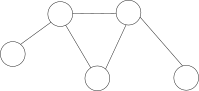
\includegraphics{undirected_graph.pdf}}\qquad	
	\subfigure[Gerichteter Graph]{\label{fig:directed_graph}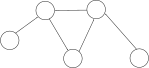
\includegraphics{directed_graph.pdf}}	
	\caption[Beispiel: Gerichteter und ungerichteter Graph]{Gerichteter und ungerichteter Graph mit $n = m = 5$.}
\end{figure}

% gewichteter Graph

\paragraph*{Gewichteter Graph} Ein gewichteter Graph (engl. \textit{weighted graph}, Abbildung \ref{fig:weighted_graph}) ist ein Tupel $G = (V,E,\omega_v,\omega_e)$. Er zeichnet sich durch die M�glichkeit aus, Gewichte an Knoten und Kanten zu definieren. Hierf�r werden die Abbildungen $\omega_v: V \rightarrow \mathbb{R}$ und $\omega_e: E \rightarrow \mathbb{R}$ verwendet.

% bezeichneter Graph
\paragraph*{Bezeichneter Graph} Ein bezeichneter Graph (engl. \textit{labeled graph}, Abbildung \ref{fig:labeled_graph}) $G=(V,E,\Sigma_{V_L},\Sigma_{E_L},\sigma_v,\sigma_e)$ erg�nzt Knoten- und Kantenmenge durch das Alphabet der Knotenbezeichner $\Sigma_{V_L}$, das Alphabet der Kantenbezeichner $\Sigma_{E_L}$ sowie die Abbildungen $\sigma_v: V \rightarrow \Sigma_{V_L}$ und $\sigma_e:E \rightarrow \Sigma_{E_L}$.

\begin{figure}[htb]
	\centering	
	\subfigure[Gerichteter, kantengewichteter Graph]{\label{fig:weighted_graph}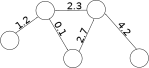
\includegraphics[scale=1.3]{weighted_graph.pdf}}\qquad	
	\subfigure[Gerichteter, bezeichneter Graph mit $\Sigma_{V_L} = \{1,2,3,4,5\}$ und $\Sigma_{E_L} = \{a,b,c,d,e\}$]{\label{fig:labeled_graph}\includegraphics[scale=1.3]{labeled_graph.pdf}}	
	\caption[Beispiel: Gewichteter und bezeichneter Graph]{Gewichteter und bezeichneter Graph.}
\end{figure}

% attributierter Graph
\paragraph*{Attributierter Graph} Ein attributierter Graph (engl. \textit{attributed graph}, Abbildung \ref{fig:attributed_graph}) verf�gt �ber die M�glichkeit, Knoten und Kanten mit zus�tzlichen Informationen in Form von Schl�ssel-Wert-Paaren zu versehen. Der Graph wird durch das Tupel \linebreak $G=(V,E,\Sigma_{V_A}, \Sigma_{E_A}, \gamma_V, \gamma_E, A)$ definiert, wobei $\Sigma_{V_A}$ das Alphabet aller m�glichen Schl�ssel f�r Knoteneigenschaften und $\Sigma_{E_A}$ jenes f�r alle Schl�ssel der Kanteneigenschaften bildet. $A$ ist die Menge der Eigenschaftswerte f�r Knoten und Kanten. Die Abbildung $\gamma_v: \Sigma_{V_A} \times V \rightarrow \mathcal P(A)$ ordnet die Knotenschl�ssel ihren entsprechenden Werten oder Wertemengen zu, gleiches gilt f�r Kanten unter Verwendung der Abbildung $\gamma_e: \Sigma_{E_A} \times E \rightarrow \mathcal P(A)$.

% Multigraph
\paragraph*{Multigraph} Ein Multigraph (Abbildung \ref{fig:multigraph}) ist ein Graph $G=(V,E)$, in dem die Menge aller Kanten $E$ eine Multimenge ist. Diese weist die Eigenschaft auf, dass einzelne Elemente mehrfach enthalten sein k�nnen. Somit ist die Definition beliebig vieler Kanten zwischen zwei Knoten m�glich. Zwei gerichtete Kanten gelten als \textit{parallel}, wenn sie den gleichen Start- und Zielknoten aufweisen.

\begin{figure}[htb]
	\centering	
	\subfigure[Knotenattributierter, gerichteter Graph mit $\Sigma_{V_A} = \{a,b\}$ und $A = \{1,2,3,4,5,h,o,d,r\}$]{\label{fig:attributed_graph}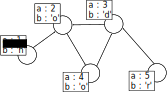
\includegraphics[scale=1.5]{attributes_graph.pdf}}\qquad	
	\subfigure[Gerichteter, kantenbezeichneter Multigraph]{\label{fig:multigraph}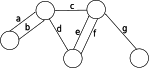
\includegraphics[scale=1.5]{multigraph.pdf}}	
	\caption[Beispiel: Attributierter Graph und Multigraph]{Attributierter Graph und Multigraph.}	
\end{figure}

Bei der Betrachtung der verschiedenen Graph-Typen wird deutlich, dass diese sich nicht zwingend gegenseitig ausschlie�en. Die Kanten in einem Multigraphen k�nnen zum Beispiel gerichtet und bezeichnet sein. Dar�ber hinaus lassen sich bezeichnete Graphen mit Hilfe von attributierten Graphen abbilden. Neben den verschiedenen Arten von Graphen sind in der vorliegenden Arbeit weitere graphentheoretische Konzepte relevant, welche im Folgenden definiert werden. Alle Definitionen beziehen sich auf gerichtete Graphen.

\paragraph*{Teilgraph, Obergraph} Ein Graph $G'=(V',E')$ hei�t Teilgraph oder Subgraph von einem Graph $G=(V, E)$, wenn $V' \subseteq V$ und $E' \subseteq E$. $G$ ist der Obergraph von $G'$. Der Teilgraph $G'$ ist \textit{induziert}, wenn er alle Kanten $(x,y) \in E$ mit $x,y \in V'$ enth�lt.

\paragraph*{Nachbarschaft} Zwei Knoten $u,v \in V$, die durch eine Kante $e = (u,v)$ verbunden sind, hei�en \textit{adjazent} oder benachbart in $G$. Die Nachbarschaft $N(v)$ eines Knotens $v$ ist die Menge aller adjazenten Knoten von $v$: 
\begin{equation}
	N(v) := \{u \mid (u,v) \in E \vee (v,u) \in E\}.
\end{equation}

\paragraph*{Au�en- und Innengrad, Grad}  Der Au�engrad $d^+(v)$ eines Knotens $v \in V$ ist die Anzahl der Kanten in $E$, deren Startknoten $v$ ist. Der Innengrad $d^-(v)$ von $v$ ist die Anzahl der in $v$ endenden Kanten. Der Grad $deg(v)$ eines Knotens $v \in V$ ist die Summe aus Au�engrad und Innengrad f�r diesen Knoten. Somit gilt in gerichteten Graphen:
\begin{equation}
	deg(v) := d^+(v)+d^-(v) = \left|N(v)\right|.
\end{equation}
In gewichteten Graphen werden bei der Berechnung des Grades die einzelnen Kantengewichte ber�cksichtigt.
\begin{equation}
	deg(v) := \sum_{e \in N(v)}\omega_e(e) 
\end{equation}

\paragraph*{Weg, Kantenfolge, Pfad, Kreis} Ein Weg ist eine Sequenz $v_1,e_1,v_2,e_2,...,v_{k-1},e_{k-1},v_k$ von Knoten und Kanten eines Graphen $G$. Die \textit{L�nge} des Weges ist die Anzahl der Kanten innerhalb der Sequenz. Ein Weg ist eine Kantenfolge in $G$, wenn jede Kante h�chstens einmal in dieser Folge auftritt. Gilt $v_1 = v_k$, so bezeichnet man diese Folge als \textit{geschlossen}, andernfalls handelt es sich um eine \textit{offene} Kantenfolge. Eine Kantenfolge ist ein Pfad, wenn alle Knoten innerhalb der Folge voneinander verschieden sind. Kommt mit Ausnahme von $v_k$ kein Knoten doppelt in der geschlossenen Kantenfolge vor, bezeichnet man diese als einfachen Kreis. Ein Graph, der einen Kreis enth�lt, ist ein zyklischer Graph.

\paragraph*{Abstand} Der Abstand $dist(u,v)$ von zwei Knoten $u,v \in V$ ist die L�nge des k�rzesten Pfades von $u$ nach $v$. Existiert kein solcher Weg, so gilt $dist(u,v) = \infty$.

\section{Arten von Netzwerken}
\label{sec:nwarten}

Netzwerk ist ein allgemeiner Oberbegriff f�r die Beschreibung von Beziehungen zwischen Objekten. Art und Verteilung der Beziehungen definieren dabei ein Muster, anhand dessen sich Aussagen �ber das Netzwerk treffen lassen. Objekte und deren Beziehungen werden mittels Knoten und Kanten modelliert und durch graphentheoretische Algorithmen analysiert. Im Folgenden werden vier verschiedene Arten von Netzwerken nach Newman\cite{Newman:2010:NI:1809753} vorgestellt.

\textbf{Technologische Netzwerke} bilden physische Infrastrukturen ab. Einer der bekanntesten Vertreter ist das Internet. Hier ist das Finden effizienter Routen, auf deren Grundlage Datenpakete zwischen Knoten weitergeleitet werden, eine der wesentlichen Aufgaben. Transportnetzwerke z�hlen ebenfalls zu den technologischen Netzwerken. Orte werden als Knoten und die Verbindungen zwischen ihnen als Kanten modelliert. Eine typische Anwendung ist auch hier das Ermitteln von Routen zwischen zwei oder mehreren Orten. Dabei ist nicht immer ausschlie�lich der geographisch k�rzeste Weg von Interesse, vielmehr spielen zus�tzliche Einschr�nkungen, wie die Kombination verschiedener Transportmittel und das Meiden bestimmter Knoten (z.B. von Gro�st�dten) eine Rolle.

In \textbf{sozialen Netzwerken} stehen die Knoten f�r Personen, Gruppen oder Ereignisse, die Kanten beschreiben Beziehungen zwischen ihnen. Diese Beziehungen k�nnen sehr vielf�ltig sein, typische Beispiele sind Freundschaft, berufliche Beziehung oder Gruppenmitgliedschaft. Prominente Beispiele sind Netzwerke, wie sie im World Wide Web zu finden sind. Hierzu z�hlen zum Beispiel Facebook\footnote{\url{http://www.facebook.com}} oder LinkedIn\footnote{\url{http://www.linkedin.com/}}. Aber auch reale soziale Netzwerke, wie zum Beispiel in Schulen oder Firmen, werden dieser Kategorie zugeordnet. Der Bereich der Social Network Analysis\cite{INSNA_web} (SNA) befasst sich mit dem Aufdecken und Analysieren von Interaktionsmustern innerhalb solcher Netzwerke. Dabei ist neben der Struktur von Organisationen und sozialen Gruppen auch die Evolution der Netzwerke von Interesse. Firmen nutzen beispielsweise Ausbreitungseigenschaften von Informationen f�r virales Marketing, auch die Verbreitungswege von Krankheiten lassen sich auf dieser Grundlage untersuchen. Des Weiteren k�nnen Empfehlungen f�r neue Kontakte oder Gruppen ausgesprochen werden. Dies erfolgt auf Basis des zur�ckliegenden Nutzerverhaltens oder der aktuellen Netzwerkstruktur in der unmittelbaren Umgebung eines Knotens.

Eine weitere Kategorie bildet die Gruppe der \textbf{biologischen Netzwerke}. In vielen Bereichen der Biologie werden Netzwerke eingesetzt um das Verhalten bestimmter Elemente abzubilden. Molekularbiologen nutzen Netzwerke um chemische Reaktionen in Zellen darzustellen, Neurowissenschaftler modellieren die Verbindungen von Hirnzellen. Eine weitere Anwendung ist die Repr�sentation des Verhaltens verschiedener Spezies in �kosystemen. 

Die vierte und f�r die vorliegende Arbeit relevante Kategorie bilden die \textbf{Informations- oder Wissensnetzwerke}, oft auch als semantische Netzwerke bezeichnet. Objekte sind dabei Informationen in Form von Begriffen oder konkreten Daten, welche miteinander verkn�pft sind. Die Beziehungen werden dabei m�glichst explizit definiert\cite{semantische_netze:2010}, lassen sich aber auch aus bestehenden Beziehungen ableiten. Bestes Beispiel f�r ein Wissensnetzwerk ist das World Wide Web. Hierbei werden Webpr�senzen als Knoten und Hyperlinks als Kanten modelliert. Kanten sind gerichtet, da eine Verbindung von Webpr�senz A zu Webpr�senz B nicht zwingend eine Verbindung von B nach A voraussetzt. Eine Wichtung der Knoten ist vorstellbar in Abh�ngigkeit des Innengrades, welcher hierbei die Anzahl der eingehenden Hyperlinks auf eine Website repr�sentiert. Diese Information wird u.a. im Pagerank\cite{Brin:1998:ALH:297805.297827} Algorithmus von Google zur Wichtung von Suchergebnissen verwendet. Eng verbunden mit dem World Wide Web ist das Semantic Web\cite{SEMWEB:2013}. Schwerpunkt ist hierbei die maschinenlesbare Repr�sentation von Beziehungen zwischen beliebigen Ressourcen.\\
Ein weiteres Informationsnetzwerk, welches auch im Rahmen aktueller Forschungen in der Abteilung Datenbanken der Universit�t Leipzig untersucht wird, sind Beziehungen innerhalb von Gesch�ftsdaten aus Gesch�ftsinformationssystemen. In diesen werden Stammdaten, wie zum Beispiel Mitarbeiter oder Produkte, mit transaktionalen Daten, wie zum Beispiel Rechnungen, Auftr�gen und Buchungen, verkn�pft. Die Instanzen der jeweiligen Datenart sind Knoten im Graphen, die Verkn�pfungen zwischen ihnen lassen sich durch bezeichnete Kanten ausdr�cken. Betrachtet man Teile dieses Graphen als Instanz eines Gesch�ftsprozesses, so kann untersucht werden, worin sich Teilgraphen erfolgreicher\footnote{Ein Prozess ist zum Beispiel genau dann erfolgreich, wenn die Summe der Einnahmen innerhalb des Prozesses die Prozesskosten �berschreitet.} Prozesse von denen nicht erfolgreicher Prozesse unterscheiden. Eine detaillierte Beschreibung des Anwendungsfalls erfolgt in Abschnitt \ref{sec:anforderungen}.

\section{Klassifikation graphenbasierter Softwaresysteme}
\label{sec:graphsystems_classification}

Aus dem vorherigen Abschnitt geht hervor, dass Graphen f�r eine Vielzahl verschiedener Anwendungen eine Rolle spielen. Daraus folgt, dass auch an die Konzeption und Implementierung dedizierter Softwaresysteme unterschiedliche Anforderungen gestellt werden. Nachfolgend werden die drei Kategorien graphenbasierter Softwaresysteme beschrieben. Die Kategorisierung gr�ndet sich auf die Ausf�hrungen in \cite{Buerli:2012}, \cite{robinson2013graph} und \cite{Shao:2012:MML:2213836.2213907} sowie eigene �berlegungen im Rahmen der Arbeit.

\subsection{Graphdatenbanksysteme}
\label{subsec:gdbms}

Kemper und Eickler definieren in \cite{kemper2006datenbanksysteme} ein Datenbankverwaltungssystem (engl. \textit{database management system}, DBMS) wie folgt:

\begin{quote}
\textit{Die Gesamtheit aller Programme zum Zugriff auf die Datenbasis, zur Kontrolle der Konsistenz und zur Modifikation der Daten wird als Datenbankverwaltungssystem bezeichnet.}
\end{quote}

Unter einer \textit{Datenbasis} versteht man die gespeicherten Daten in Form von miteinander in Beziehung stehenden Informationseinheiten. 

Angles definiert in \cite{Angles:2008} ein Graphdatenbankmodell wie folgt:

\begin{quote}
\textit{Ein Graphdatenbankmodell ist ein Modell, in welchem die Datenstrukturen f�r Schema und/oder Instanzen direkt als Graph modelliert sind. Datenmanipulation erfolgt durch graphenorientierte Operationen und Typkonstruktoren, Integrit�tsbedingungen k�nnen auf der Graphstruktur definiert werden.}
\end{quote}

Ein Datenbankverwaltungssystem, welches ein Graphdatenbankmodell implementiert, wird im Rahmen dieser Arbeit als \textbf{Graphdatenbankverwaltungssystem} (engl. \textit{graph database management system}, GDBMS) bezeichnet. Eine \textit{Graphdatenbank} ist die Instanz eines Graphen und stellt somit die vom GDBMS verwaltete Datenbasis dar. 
%Der von Angles verwendete Begriff der Datenstruktur wird allgemeiner als \textit{Datenmodell} bezeichnet (Abschnitt \ref{sec:datamodels}). 
Nachfolgend werden die Begriffe Graphdatenbanksystem und Graphdatenbankverwaltungssystem im Text synonym verwendet.

Graphdatenbanksysteme sind generell f�r den Einsatz als OLTP-System (engl. \textit{Online Transaction Processing}) konzipiert\cite{robinson2013graph}. Der Schwerpunkt liegt somit auf Mehrbenutzerf�higkeit, transaktionaler Performance, Integrit�t und Verf�gbarkeit. GDBMS eignen sich vorrangig f�r die Ausf�hrung lokaler Operationen, diese betrachten nur einen Teil des Graphen, wie zum Beispiel die Umgebung eines definierten Knotens oder einer Knotenmenge.

Festzuhalten ist, dass sich ein GDBMS �ber drei wesentliche Aufgaben definiert:
\begin{enumerate}
	\item Bereitstellen von Informationen als Instanz eines graphenspezifischen Datenmodells
	\item Bereitstellen von Operationen zur Definition, Manipulation und Abfrage einer Instanz des Datenmodells
	\item Sicherstellen der Widerspruchsfreiheit innerhalb der Datenbasis
\end{enumerate}

Ausgehend von dieser allgemeinen Definition lassen sich die vorhandenen Systeme weiter unterteilen. Nachfolgend werden die im Rahmen der Arbeit relevanten Auspr�gungen von GDBMS erl�utert.

\paragraph*{Native versus nicht-native GDBMS}

Als native GDBMS bezeichnet man jene Systeme, in denen sowohl die Verarbeitung als auch die Speicherung der Datenbasis graphenorientiert erfolgt\cite{robinson2013graph}. Im Sinne der Verarbeitung spielt hierbei das Konzept der \textit{indexfreien Adjazenz}\cite{DBLP:journals/corr/abs-1004-1001} eine entscheidende Rolle. Zum Verst�ndis soll kurz die Modellierung von Netzwerken im relationalen Datenmodell\cite{Codd:1970:RMD:362384.362685} skizziert werden. In RDBMS werden Beziehungen zwischen Objekten durch Fremdschl�sselattribute und im Fall von $n:m$ Beziehungen durch zus�tzliche Tabellen (engl. \textit{mapping tables}) abgebildet. Im Zuge der Normalisierung entsteht eine gro�e Anzahl von Tabellen, welche �ber Fremdschl�sselbeziehungen miteinander verbunden sind. F�r die Verwaltung stark vernetzter Daten weist dieses Modell einen entscheidenden Nachteil auf: Im Falle einer Selektion m�ssen die Tabellen unter der Verwendung von Verbundoperationen (sog. JOIN-Operationen) wieder zusammengef�hrt werden, um die angeforderte Teilmenge zu extrahieren. Relationale Datenbanken begegnen diesem Problem mittels Anfrageoptimierung, dem Einsatz von Cachingstrategien oder der Verwendung von Indizes auf Fremdschl�sselattributen\cite{DBLP:books/sp/HarderR01}. Der Aufwand, einen Index nach einem bestimmten Schl�ssel zu durchsuchen steht meist in einem logarithmischen Verh�ltnis zur Anzahl der hinterlegten Eintr�ge. Der Aufwand vervielfacht sich, wenn mehrere JOIN-Operationen rekursiv hintereinander ausgef�hrt werden m�ssen.\\
Native GDBMS hingegen bilden die Daten in ihrer expliziten Struktur ab, Beziehungen zwischen Objekten werden durch Kanten modelliert und als physische Referenz direkt am Objekt abgelegt. Der geringe Aufwand, die Nachbarschaft eines Knotens zur Laufzeit abzufragen, ist der entscheidende Vorteil, den diese Struktur aufweist. W�hrend bei einer JOIN-Operation typischerweise ein Index in die Berechnung einbezogen wird, ist die Komplexit�t dieser Operation in einem nativen GDBMS nur vom aktuellen Knotengrad abh�ngig. Somit bleibt sie unabh�ngig von der Gr��e des Graphen konstant. Die Kanten innerhalb des Graphen k�nnen als materialisiertes Ergebnis einer JOIN-Operation verstanden werden. Gegen�ber einem relationalen DBMS verspricht dieser Ansatz insbesondere bei rekursiven Anfragen gro�er Tiefe, wie zum Beispiel der Pfadsuche, einen entscheidenden Geschwindigkeitsvorteil.

Die M�glichkeit zur nativen Verarbeitung ist eng verkn�pft mit der Repr�sentation des Graphen im Hauptspeicher und auf Externspeichern. Eine hohe Performance rekursiver Anfragen kann nur erreicht werden, wenn der direkte Zugriff auf die Nachbarschaft eines Knotens auch physisch effizient m�glich ist. Native GDBMS speichern den Graphen in einem Format, dass f�r rekursive Operationen optimiert ist. In \cite{Shao:2012:MML:2213836.2213907} wird diskutiert, dass es keine Repr�sentation des Graphen geben kann, welche f�r alle vorstellbaren Graphalgorithmen optimal ist, da Zugriffe innerhalb des Graphen grunds�tzlich wahlfrei sind. Ungeachtet dessen existieren verschiedene Datenformate zur effizienten Verarbeitung des Graphen, diese sind jedoch nur hinsichtlich bestimmter Operationen optimiert.

Nicht-native GDBMS sind jene Systeme, welche die Modellierung der Daten als Graph unterst�tzen, f�r die Verarbeitung und Speicherung jedoch auf andere Technologien zur�ckgreifen. Dazu z�hlen zum Beispiel relationale und objektorientierte Datenbanken aber auch dedizierte Persistenzframeworks\cite{robinson2013graph}. Nicht-native GDBMS weisen den Vorteil auf, dass viele der zugrundeliegenden Systeme durch eine lange Entwicklungsdauer und den oft mehrj�hrigen Einsatz als Produktivsystem eine hohe Stabilit�t aufweisen und deren Funktionsweise umfassend dokumentiert ist. Nicht-native Verarbeitung weist bei traversierenden Anfragen Leistungsdefizite auf, daf�r k�nnen andere Anfragen, wie zum Beispiel mengenorientierte, von einer entsprechend optimierten Verarbeitung profitieren.

\paragraph*{Zentrale versus verteilte GDBMS} 

Ein weitere Differenzierung von GDBMS ist die klassische Einteilung in zentrale und verteilte Systeme. Zentrale GDBMS werden auf einem einzelnen, zentralen Rechner ausgef�hrt. Steigenden bzw. generell hohen Anforderungen hinsichtlich Anfragelast und verwalteter Datenmenge kann in diesen Systemen durch \textit{vertikale Skalierung} (engl. \textit{scale up}) begegnet werden\cite{DBLP:journals/corr/cs-AR-9912010}. Hierbei wird durch das �ndern der Hardwarekonfiguration, wie zum Beispiel dem Hinzuf�gen mehrerer, leistungsf�higerer Prozessoren oder gr��erer Mengen an Hauptspeicher, die Leistung des Systems gesteigert. Die maximale Leistungsf�higkeit ist damit durch die technische Entwicklung im Bereich der Hardware und durch die Wirtschaftlichkeit der eingesetzten Ressourcen limitiert.

Ein Weg, der Forderung nach hoher Leistungsf�higkeit zu begegnen, ist der Einsatz verteilter GDBMS. Diese zeichnen sich dadurch aus, dass Instanzen eines konkreten GDBMS auf mehreren Rechnern parallel ausgef�hrt werden. F�r die Beantwortung von Anfragen und die Verwaltung der Datenbasis kooperieren die einzelnen Instanzen. Eine Steigerung der Leistungsf�higkeit wird durch das Hinzuf�gen zus�tzlicher Rechner oder Instanzen erreicht. Dieses Vorgehen wird als \textit{horizontale Skalierung} (engl. \textit{scale out}) bezeichnet\cite{DBLP:journals/corr/cs-AR-9912010}. Ziel dabei ist eine lineare Steigerung der Leistungsf�higkeit in Abh�ngigkeit zur Anzahl der hinzugef�gten Rechner\cite{rahm1994mehrrechner}. 
%Die f�r die vorliegende Arbeit relevanten GDBMS implementieren eine \textit{shared-nothing}-Architektur, diese zeichnet sich durch einen lose gekoppelten Rechnerverbund aus, in dem jedem beteiligten Rechner eigene Hardware-Ressourcen zur Verf�gung stehen\cite{rahm1994mehrrechner}.

Bei der Aufteilung der Datenbasis in verteilten Systemen unterscheidet man zwei Techniken: \textit{Replikation} und \textit{Partitionierung}. Im Rahmen einer vollst�ndigen Replikation wird die gesamte Datenbasis an allen beteiligten Rechnern redundant hinterlegt. Dies erh�ht die Verf�gbarkeit des Gesamtsystems und erm�glicht das horizontale Skalieren lesender Zugriffe. Vollst�ndige Replikation weist den Nachteil auf, dass die Datenmenge durch die Kapazit�t der einzelnen Rechner limitiert ist.\\
Die Partitionierung teilt die Datenbasis in mehrere Fragmente auf, diese werden den beteiligten Rechnern zugewiesen. Die Folgen sind eine horizontale Skalierbarkeit schreibender Zugriffe und eine theoretisch unbeschr�nkte Gr��e der Datenbasis. Mit dem Ziel, beide Zugriffsarten skalieren und gleichzeitig Verf�gbarkeit sicherstellen zu k�nnen, werden die Fragmente im Rahmen der partiellen Replikation redundant gespeichert\cite{rahm1994mehrrechner}.

\paragraph*{Eingebettete versus Client-Server GDBMS}

Viele der aktuell verf�gbaren GDBMS k�nnen als eingebettete Datenbanksysteme verwendet werden. Die Einbettung erfolgt in Form spezieller Softwarebibliotheken innerhalb des Anwendungsprogramms, die Funktionen des GDBMS k�nnen �ber herstellerspezifische APIs in Anspruch genommen werden. Eingebettete Datenbanksysteme eignen sich insbesondere f�r den Einsatz in speziellen Ger�ten oder eigenst�ndigen Desktopanwendungen. Das Anwendungsprogramm �bernimmt die Verantwortung �ber das GDBMS, eine manuelle Installation oder Aktualisierung ist nicht erforderlich. Ein wesentlicher Vorteil der eingebetteten Verwendung ist die geringe Latenz beim Aufruf von Datenbankfunktionen. Ein m�glicher Nachteil ist die Bindung an den Prozess des Anwendungsprogramms, mit welchem sich das GDBMS Ressourcen, wie zum Beispiel den verf�gbaren Hauptspeicher, teilen muss. Ein weiterer Nachteil ist die Einschr�nkung in der Wahl der Programmiersprache, da die Softwarebibliotheken typischerweise nur in der Programmiersprache des jeweiligen GDBMS zur Verf�gung stehen.

Neben der Einbettung in das Anwendungsprogramm bieten viele GDBMS-Hersteller auch die Verwendung eines eigenst�ndigen Datenbankservers an. Generell werden Datenbanksysteme h�ufig als Client-Server-Systeme realisiert\cite{vossen2008datenmodelle}. Ein Client sendet eine Anfrage an einen Server, dieser bearbeitet die Anfrage und sendet eine Antwort an den Client zur�ck. Client- und Serverprozess sind entkoppelt, was zur Folge hat, dass mehrere Clients gleichzeitig mit dem Server kommunizieren k�nnen. Die Kommunikation erfolgt auf Basis der Protokolle des jeweiligen Datenbanksystems. Viele Graphdatenbanksysteme nutzen standardisierte Protokolle f�r die Kommunikation zwischen Client und Server. Infolgedessen ist die Verwendung des GDBMS grunds�tzlich unabh�ngig von Plattform und Programmiersprache. Ein Nachteil der Client-Server-Architektur ist die h�here Latenz durch den zus�tzlichen Kommunikationsaufwand. Dar�ber hinaus zieht der Einsatz eines Datenbankservers auch entsprechende administrative Aufgaben nach sich.

\paragraph*{Disk- versus hauptspeicher-zentrierte GDBMS}

Ein weiteres wichtiges Unterscheidungsmerkmal zwischen GDBMS-Implementierungen ist die Wahl des prim�ren Speichermediums f�r die hinterlegten Daten. Generell wird in disk-zentrierte (engl. \textit{disk resident}) und hauptspeicher-zentrierte (engl. \textit{main memory based} oder \textit{in-memory}) DBMS unterschieden\cite{Garcia-Molina:1992:MMD:627289.627538}.

Disk-zentrierte DBMS stellen die klassische Form eines Datenbanksystems dar. Ihre Entwicklung erfolgte unter der Vorgabe, dass die gesamte Datenbasis auf mechanischen Festplatten hinterlegt und einzelne Fragmente bei Bedarf zur Verarbeitung in den Hauptspeicher geladen werden. Die Zugriffszeiten des Hauptspeichers sind wesentlich k�rzer als die von Festplatten. Ein wahlfreier Zugriff auf die Informationen im Hauptspeicher ist demnach effizienter als das wahlfreie Lesen von Daten auf den rotierenden Magnetscheiben einer Festplatte. DBMS-Hersteller begegneten diesem Problem mit sequentieller, an der Blockstruktur der Festplatten orientierten Datenspeicherung und dem Einsatz gro�er Datenbankpuffer mit entsprechenden Ersetzungsverfahren\cite{DBLP:books/sp/HarderR01}.

Hauptspeicher-zentrierte DBMS verwalten die gesamte Datenbasis innerhalb des physischen Hauptspeichers. Die eingesetzten Algorithmen und Datenstrukturen sind auf die Kommunikation zwischen Hauptspeicher, Prozessor-Caches und CPU-Registern optimiert. Durch die geringen Zugriffszeiten wird weniger die sequentielle Anordnung der Daten priorisiert, vielmehr wird versucht, durch Komprimierung mehr Daten im Hauptspeicher verwalten zu k�nnen\cite{plattner2011memory}. Hauptspeicher-zentrierte Verarbeitung ist nicht gleichbedeutend mit der Verwendung gro�er Puffer, welche den gesamten Datenbestand eines disk-zentrierten Systems aufnehmen k�nnen. Der Puffer stellt eine zus�tzliche Indirektion im Zugriff dar, Adressen m�ssen �bersetzt, das Vorhandensein des entsprechenden Blocks im Puffer gepr�ft und das angeforderte Tupel letztendlich ausgelesen werden. Diese Schritte entfallen bei einer hauptspeicher-zentrierten Verarbeitung.

Ein wesentlicher Nachteil des Hauptspeichers ist dessen Fl�chtigkeit. Wird die Stromversorgung unterbrochen, sind die hinterlegten Informationen verloren. Die Systeme nutzen zwar den Hauptspeicher als prim�res Speichermedium, setzen jedoch h�ufig Externspeicher f�r Backups ein. Insbesondere die Verwendung von Solid-State-Disks (SSD) bietet hier wesentliche Performance-Vorteile gegen�ber mechanischen Festplatten. 
%Durch die Wirtschaftlichkeit gro�er Mengen an Hauptspeicher erlangen In-Memory-DBMS zunehmend an Bedeutung. 
Wie bereits erw�hnt, erfolgt der Zugriff innerhalb des Graphen grunds�tzlich wahlfrei. Infolgedessen stellen hauptspeicher-zentrierte Implementierungen vor allem im Bereich der GDBMS eine interessante Alternative dar.

Die vorgestellten Auspr�gungen von Graphdatenbanksystemen schlie�en sich nicht zwingend gegenseitig aus, Kombinationen der einzelnen Arten sind m�glich. So ist es vorstellbar, dass ein hauptspeicher-zentriertes GDBMS als Client-Server-System eingesetzt wird oder native GDBMS in Desktopanwendungen eingebettet sind.

\subsection{Graph Processing Systems}
\label{subsec:graph_processing}

Eine zweite Art graphenbasierter Softwaresysteme sind diejenigen, welche sich mit der verteilten Analyse umfangreicher Graphen befassen. Sie werden als Graph Processing Systems (GPS) oder alternativ auch als Graph Compute Systems bezeichnet\cite{Malewicz:2010:PSL:1807167.1807184, robinson2013graph}. Ein umfangreicher Graph weist die Eigenschaft auf, dass seine Knoten- und Kantenmenge nicht mehr effizient auf einer einzelnen Maschine verarbeitet werden kann.

Anders als Graphdatenbanksysteme eignen sich GPS f�r Berechnungen, welche den gesamten Graphen ber�cksichtigen. Ein Beispiel hierf�r ist der Page-Rank-Algorithmus\cite{Brin:1998:ALH:297805.297827} von Google, welcher jeder Website einen globalen Rang auf Basis ihrer Nachbarschaft und weiteren Faktoren zuweist. Bei der Analyse sozialer Netzwerke ist zum Beispiel die Berechnung der Zentralit�t eines Knotens interessant: F�r jedes m�gliche Nutzerpaar werden die k�rzesten Pfade bestimmt um anschlie�end den Anteil jener Pfade zu berechnen, welche durch einen konkreten dritten Nutzer verlaufen.

Eine weitere Eigenschaft dieser Systeme ist die batch-orientierte Datenverarbeitung. Die Daten werden von einer externen Quelle geladen, auf mehrere Rechner verteilt, verarbeitet und das Ergebnis der Verarbeitung ausgegeben oder aber in einer nachfolgenden Berechnung weiterverwendet. Dies ist ein wesentlicher Unterschied zur Definition eines operationalen Graphdatenbanksystems, welches die Datenbasis selbst verwaltet, den interaktiven Zugriff erm�glicht und Konsistenz sicherstellt. Durch die batch-orientierte Verarbeitung k�nnen GPS eher mit OLAP-Systemen (engl. \textit{online analytical processing}) verglichen werden.

GPS werden im Rahmen dieser Arbeit nicht betrachtet, da ihr Einsatzzweck nicht zu den gestellten Anforderungen passt. Hierzu z�hlen u.a. der interaktive Zugriff und der lokale Bezug von Anfragen. Bekannte GPS-Vertreter sind die quelloffenen Projekte Apache Giraph\footnote{\url{http://giraph.apache.org/}} und Phoebus\footnote{\url{https://github.com/xslogic/phoebus}}. Beide Systeme implementieren das von Google vorgestellte Pregel-Modell\cite{Malewicz:2010:PSL:1807167.1807184}, welches unter anderem f�r die Berechnung des Page-Rank-Algorithmus eingesetzt wird und im Gegensatz zu anderen Systemen Ausf�lle von Rechnern w�hrend der Verarbeitung toleriert. MapReduce\cite{Dean:2008:MSD:1327452.1327492} ist ebenfalls ein verteiltes Berechnungsmodell f�r gro�e Datenmengen. Apache Hadoop\footnote{\url{http://hadoop.apache.org/}} ist eine bekannte Implementierung des Modells und wird im Rahmen des Pegasus-Projektes\footnote{\url{http://www.cs.cmu.edu/~pegasus/}} f�r die Berechnung von Graphalgorithmen auf umfangreichen Graphen eingesetzt.

\subsection{Software zur Analyse und Visualisierung}

Die dritte Kategorie graphenbasierter Softwaresysteme bilden unterst�tzende Werkzeuge zur Analyse und bzw. oder Visualisierung von Graphen. Es handelt sich um zentral ausf�hrbare oder als Softwarebibliothek verwendbare Programme. Die Gr��e der unterst�tzten Graphen ist durch die zur Verf�gung stehende Menge an Hauptspeicher begrenzt. Die Systeme selbst bieten keine Unterst�tzung f�r eine automatische Datenverwaltung, Mehrbenutzerf�higkeit oder Konsistenzerhaltung an. Der analytische Funktionsumfang variiert je nach System, so werden typischerweise die Berechnung globaler Eigenschaften, wie zum Beispiel die Dichte\footnote{Die Dichte eines Graphen beschreibt das Verh�ltnis zwischen der Anzahl von Kanten und der maximal m�glichen Anzahl von Kanten\cite{DBLP:books/daglib/0030488}.} des Graphen, der durchschnittliche Grad oder die Anzahl maximal zusammenh�ngender Teilgraphen\footnote{Ein Graph ist zusammenh�ngend, wenn alle m�glichen Knotenpaare innerhalb des Graphen durch einen Weg verbunden sind\cite{DBLP:books/daglib/0030488}.} genauso unterst�tzt wie lokale Operationen. Letztere umfassen zum Beispiel das Berechnen k�rzester Pfade oder maximaler Fl�sse.

Die Visualisierung von Graphen stellt ebenfalls ein wichtiges Forschungsgebiet dar\cite{kaufmann2001drawing}. Die grafische Aufbereitung komplexer Netzwerke kann dem Endanwender das Verst�ndnis erleichtern und auch neue Erkenntnisse �ber Eigenschaften oder Besonderheiten des Graphen erm�glichen. Verschiedene Layout-Algorithmen werden in den jeweiligen Systemen implementiert, um je nach Topologie des Graphen die optimale Visualisierung w�hlen zu k�nnen. Einige der Systeme stellen Erweiterungen f�r die Kommunikation mit GDBMS zur Verf�gung, wodurch die im Datenbanksystem hinterlegten Daten visualisiert werden k�nnen.

Die dritte Kategorie graphenbasierter Softwaresysteme wird im Rahmen der vorliegenden Arbeit nicht betrachtet, da die Systeme f�r die dauerhafte Datenverwaltung ungeeignet sind. Beispiele f�r Softwaresysteme zur Analyse und Visualisierung sind JUNG\footnote{\url{http://jung.sourceforge.net/}}, GraphViz\footnote{\url{http://www.graphviz.org/}} und Gephi\footnote{\url{https://gephi.org/}}.

\section{Datenmodelle in GDBMS}
\label{sec:datamodels}

Datenbankmanagementsysteme implementieren ein Datenmodell, welches die Modellierungskonstrukte festlegt, mittels derer ein Informationsabbild der realen Welt generiert werden kann. Ein Datenbankmodell ist somit eine Form der Abstraktion und bietet die M�glichkeit zur Modellierung von Datenobjekten und zur Festlegung der anwendbaren Operatoren und deren Wirkung\cite{elmasri2009grundlagen, kemper2006datenbanksysteme}. Die in GDBMS h�ufig eingesetzten Datenmodelle sind das Property-Graph-Modell und das Hypergraph-Modell. Im Bereich des Semantic Web findet das Resource Description Framework zur Modellierung von Graphen Anwendung.

\subsection{Property-Graph-Modell}
\label{subsec:propgraph}

Das Property-Graph-Modell (PGM) ist ein gerichteter, kantenbezeichneter, attributierter Multigraph\cite{DBLP:journals/corr/abs-1006-2361, DBLP:journals/corr/abs-1004-1001}. Formal betrachtet l�sst sich dieser als ein Tupel in der Form \linebreak$G = (V,E,\Sigma_{E_L}, \Sigma_{V_A}, \Sigma_{E_A}, A, \sigma_e, \gamma_v, \gamma_e)$ definieren. $\Sigma_{E_L}$ beschreibt das Alphabet der Kantenbezeichner, dessen Symbole durch die Abbildung $\sigma_e:E \rightarrow \Sigma_{E_L}$ den Kanten zugeordnet werden. $\Sigma_{V_A}$ bzw. $\Sigma_{V_E}$ bilden die Schl�sselalphabete, $A$ die Wertemenge f�r Knoten- bzw. Kantenattribute. Die Abbildungen $\gamma_v: \Sigma_{V_A} \times V \rightarrow \mathcal P(A)$ und $\gamma_e: \Sigma_{V_E} \times E \rightarrow \mathcal P(A)$ ordnen die Knotenschl�ssel ihren entsprechenden Werten oder Wertemengen zu. 

Gro�er Vorteil des PGM ist dessen Flexibilit�t hinsichtlich der Abbildung verschiedener Arten von Graphen\cite{DBLP:journals/corr/abs-1006-2361}. Neben der grundlegenden ungerichteten Form ohne zus�tzliche Eigenschaften, l�sst sich jede Kombination aus gerichteten, gewichteten und attributierten Graphen und Multigraphen darstellen. Das Modell eignet sich somit zur Repr�sentation einer Vielzahl der im vorhergehenden Abschnitt vorgestellten Netzwerke.

Das Modell sieht keine strenge Typisierung von Knoten und Kanten vor, d.h. deren Attribute sind grunds�tzlich nicht durch ein Schema festgelegt und k�nnen damit beliebig auf Instanzebene vergeben werden. Es handelt sich demnach um ein semistrukturiertes Modell, da keine explizite Unterscheidung zwischen Strukturinformationen und Daten vorgenommen wird, sondern vielmehr jede Instanz eines Knotens bzw. einer Kante die jeweiligen Informationen in sich vereint. Der sich daraus ergebende Vorteil ist die hohe Flexibilit�t zum Einen gegen�ber der Schemaevolution an Knoten und Kanten innerhalb des Modells und zum Anderen im Datenaustausch zwischen verschieden modellierten Datenquellen. In diversen Anwendungen kann es jedoch sinnvoll sein, den Typ eines Knotens zu modellieren. Auf logischer Ebene erlaubt dies eine semantisch eindeutige Beschreibung der einzelnen Instanzen, auf physischer Ebene die Definition von Indizes und Konsistenzkriterien oder die Ber�cksichtigung des Typen im Rahmen der Anfrageoptimierung\cite{EdlichFriedlandHampeBrauer201010}. Eine M�glichkeit der Realisierung ist der Einsatz dedizierter Attributschl�ssel, wie zum Beispiel \texttt{Type}. Die Zust�ndigkeit f�r Definition und Einhaltung eines Schemas liegt in diesem Fall bei der Anwendung. Einige GDBMS bieten die M�glichkeit Knoten- und Kantentypen zu definieren und �bernehmen somit ihrerseits die Verantwortung f�r die Einhaltung anwendungsspezifischer und modellinh�renter Integrit�tsbedingungen.

Abbildung \ref{fig:propertygraph} zeigt am Beispiel eines sozialen Netzwerkes die Instanz eines Property-Graphen. Personen stehen miteinander �ber Freundschaften in Beziehung, studieren an Hochschulen oder sind Mitglied in Vereinen, die wiederum von Hochschulen betreut werden. Knotenattribute werden in der Form \texttt{Schl�ssel : Wert} dargestellt. Die Knotentypen Hochschule, Person und Verein sind farblich voneinander abgehoben, der jeweilige Typ wird durch den Attributschl�ssel \texttt{Type} definiert. Das Beispiel verzichtet auf Kantenattribute, vorstellbar w�ren aber zum Beispiel die Rolle einer Person in einem Verein oder Datumsangaben, welche den Erstellungszeitpunkt der Beziehung dokumentieren.

\begin{figure}[htb] 
	\centering
		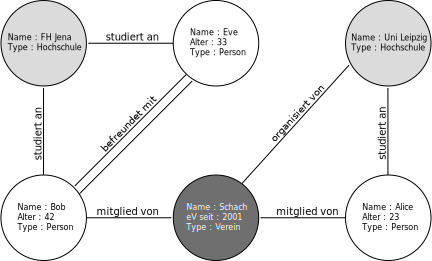
\includegraphics{PropertyGraph.pdf}
	\caption[Beispiel: Property-Graph]{Beispiel eines Property-Graphen mit den drei Knotentypen Hochschule, Verein und Person, welche �ber verschiedene Kantentypen in Relation miteinander stehen.}
	\label{fig:propertygraph}
\end{figure}

Bis auf wenige Ausnahmen wird das Property-Graph-Modell in nahezu allen kommerziell verf�gbaren GDBMS eingesetzt\cite{EdlichFriedlandHampeBrauer201010}. Teilweise wird das Modell modifiziert, ein Beispiel hierf�r sind explizite Knotenbezeichner in Neo4j 2.0\cite{Neo4j_web_labels:2013}.

\subsection{Hypergraph-Modell}
\label{subsec:hgm}

Die zu Beginn des Kapitels betrachteten Graphen-Definitionen sowie das PGM erlauben ausschlie�lich bin�re Beziehungen zwischen Objekten, d.h. eine Kante verbindet genau zwei Knoten. Es existieren jedoch Anwendungsgebiete, in denen die Modellierung von n-�ren Beziehungen von Interesse ist. Ein Beispiel hierf�r ist die Wissensrepr�sentation, welche unter anderem in den Bereichen k�nstliche Intelligenz, Bioinformatik und Computerlinguistik eingesetzt wird\cite{Iordanov:2010:HGG:1927585.1927589}. Grunds�tzlich lassen sich n-�re Beziehungen durch mehrere bin�re Relationen ausdr�cken. Dies erh�ht jedoch die Komplexit�t und Fehleranf�lligkeit der Repr�sentation und verringert gleichzeitig deren Verst�ndlichkeit und �bersichtlichkeit. In Hypergraphen wird von dieser Komplexit�t abstrahiert, indem mehrere bin�re Relationen in Hyperkanten zusammengefasst werden.

Das Hypergraph-Modell (HGM) beschreibt einen Hypergraph $H=(V,E)$ bestehend aus einer Menge $V=\{v_1,v_2,\ldots,v_n\}$ von Knoten und einer Menge $E = \{E_1,E_2,\ldots E_m\} = \mathcal P(V) \setminus \emptyset$ von Hyperkanten, wobei $E_i \subseteq V$ f�r $i=1,\ldots,m$. Eine gerichtete Hyperkante ist ein geordnetes Paar $E = (A,B)$ mit $A,B \subseteq V$ und $A \cap B = \emptyset$. Ein gerichteter Hypergraph besteht aus gerichteten Hyperkanten\cite{Gallo:1993:DHA:153578.153586}.

\begin{figure}[htb] 
	\centering
		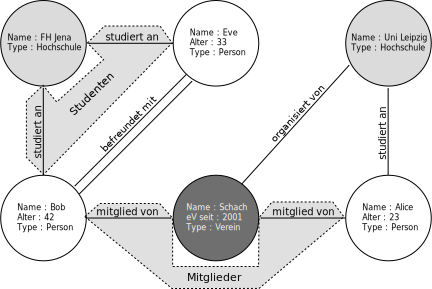
\includegraphics{PropertyHyperGraph.pdf}
	\caption[Beispiel: Property-Hypergraph]{Beispiel eines Property-Hypergraphen mit zwei gerichteten Hyperkanten $\texttt{Studenten} = (\{\texttt{Eve}, \texttt{Bob}\}, \{\texttt{FH Jena}\})$ und $\texttt{Mitglieder} = (\{\texttt{Alice}, \texttt{Bob}\}, \{\texttt{Schach}\})$.}
	\label{fig:propertyhypergraph}
\end{figure}

Abbildung \ref{fig:propertyhypergraph} greift das Beispiel des sozialen Netzwerkes erneut auf. Die bin�ren Relationen \texttt{studiert an} und \texttt{mitglied von} werden zu den gerichteten Hyperkanten \texttt{Studenten} und \texttt{Mitglieder} zusammengefasst. Knoten, Kanten und Hyperkanten k�nnen auch in Hypergraphen mit Attributen und Bezeichnern versehen werden. Ein Property-Graph-Modell mit der M�glichkeit, n-�re Beziehungen zu definieren, wird als Property-Hypergraph-Modell (PHGM) bezeichnet und weist die gleichen Eigenschaften bez�glich Strukturiertheit bzw. Typisierung wie das PGM auf.

Im Vergleich zum PGM ist das HGM in kommerziellen GDBMS wenig verbreitet. Ein Vertreter ist das Graphdatenbanksystem HyperGraphDB, welches das HGM um ein flexibles Typsystem und die M�glichkeit Hyperkanten auf Hyperkanten zeigen zu lassen erweitert\cite{Iordanov:2010:HGG:1927585.1927589}.

\subsection{Resource Description Framework}
\label{subsec:rdf}

Das Resource Description Framework\cite{RDF:2013} (RDF) ist ein vom World Wide Web Consortium (W3C) standardisiertes Datenmodell f�r die Formulierung und den Austausch von Aussagen �ber beliebige Dinge, welche innerhalb des Modells als Ressourcen bezeichnet werden. RDF wurde im Umfeld des Semantic Web\cite{SEMWEB:2013} entwickelt, dieses widmet sich der semantischen Auszeichnung von Informationen und deren maschineller Interpretation und Verarbeitung.

Eine Aussage ist als ein Tripel bestehend aus Subjekt, Pr�dikat und Objekt definiert. Das Subjekt ist die zu beschreibende Ressource, das Pr�dikat definiert eine Eigenschaft des Subjektes und das Objekt den Wert dieser Eigenschaft. Pr�dikate sind ebenfalls Ressourcen, Objekte k�nnen entweder Ressource oder Literal sein. Eine Menge von Aussagen zu einem Subjekt bildet somit dessen Beschreibung. Eine Ressource wird durch einen Uniform Resource Identifier (URI) eindeutig identifiziert. F�r die automatisierte maschinelle Verarbeitung ist diese Eindeutigkeit obligatorisch, da sie Mehrdeutigkeiten und folglich Fehlinterpretationen verhindert\cite{DBLP:journals/dlib/Miller98}. 

Aus mathematischer Sicht betrachtet ist das RDF-Modell ein gerichteter, bezeichneter Multigraph. Ein wesentlicher Unterschied zum PGM besteht darin, dass Knoten- und Kanteneigenschaften durch dedizierte Tripel modelliert werden m�ssen. Eine modellinh�rente Differenzierung in eine Beziehung zwischen Ressourcen und einer Beschreibung einer einzelnen Ressource ist dabei nicht gegeben. Das Modell erfordert keine strenge Typisierung und eignet sich somit genau wie PGM und HGM f�r die Speicherung semistrukturierter Daten. Abbildung \ref{fig:rdfgraph} zeigt dies am Beispiel eines sozialen Netzwerkes.

\begin{figure}[htb] 
	\centering
		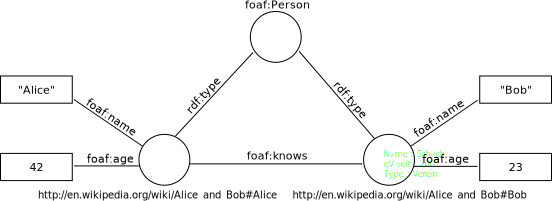
\includegraphics{RDFGraph.pdf}
	\caption[Beispiel: RDF-Instanz]{Instanz eines RDF-Modells am Beispiel eines sozialen Netzwerkes. Gezeigt werden die Ressourcen Alice  und Bob, welche durch die entsprechenden Wikipedia-URIs eindeutig bestimmt sind. Ihre Beziehung wird durch das Pr�dikat \texttt{foaf:knows} beschrieben. Beide Ressourcen sind vom Typ \texttt{foaf:Person}. Die Beziehungen selbst sind ebenfalls Ressourcen, Friend-of-a-friend (\texttt{foaf}) repr�sentiert den Namensraum \texttt{http://xmlns.com/foaf/spec/}, das Prefix \texttt{rdf} den Namensraum \texttt{http://www.w3.org/1999/02/22-rdf-syntax-ns\#}. Die Beschreibung von Alice und Bob wird durch deren Beziehungen zu den Literalen \texttt{Alice} und \texttt{42} bzw. \texttt{Bob} und \texttt{23} erg�nzt.}
	\label{fig:rdfgraph}
\end{figure}

F�r die Manipulation und den Zugriff auf Daten im RDF-Modell wird die graphenbasierte Anfragesprache SPARQL\cite{SPARQL:2013} entwickelt und eingesetzt. Deren grundlegender Ansatz ist die Definition eines Teilgraphen als Muster, nach welchem die Datenbasis durchsucht wird. Innerhalb des Musters k�nnen Variablen definiert werden, diese werden w�hrend der Anfrageverarbeitung instanziiert. Wird das Muster in der Datenbasis gefunden, besteht die Ergebnismenge aus den definierten Variablen und deren Belegung.

Einer der Schwerpunkte des Semantic Web ist das Ableiten neuer Beziehungen zwischen Ressourcen auf der Basis vorhandener Informationen und zus�tzlich definierter Regeln. Dieses Vorgehen wird auch als Inferenz bezeichnet\cite{Inference:2013}. Ein zweiter Schwerpunkt ist das Konzept des Linked Data\cite{linked_data:2013}. Es beschreibt, wie eigenst�ndige Datenquellen im Web virtuell zusammengef�hrt und quellen�bergreifende Beziehungen zwischen den Ressourcen definiert werden. Mit Hilfe dieser umfassenden,  virtuell integrierten Datenbasis k�nnen komplexe Anfragen beantwortet und neue Informationen abgeleitet werden.

F�r die Speicherung von RDF-Daten werden entweder spezielle Datenbanksysteme, sog. Triple-Stores, eingesetzt oder aber bestehende Datenbanksysteme, wie zum Beispiel \linebreak RDBMS, mit entsprechender Funktionalit�t erweitert. Beide Systemarten unterst�tzen nicht die im vorhergehenden Abschnitt definierte indexfreie Adjazenz und z�hlen somit zu den nicht-nativen GDBMS\cite{robinson2013graph}. Die Systeme selbst bieten SPARQL-Endpunkte an, �ber welche auf die hinterlegte Datenbasis zugegriffen werden kann.

Das RDF-Modell und SPARQL geh�ren zu den grundlegenden Komponenten des Semantic Web. Wie bereits erw�hnt, sind die wesentlichen Einsatzszenarien das Ableiten neuer Beziehungen und das virtuelle Integrieren von Daten aus verschiedenen Quellen. Diese Szenarien sind jedoch nicht wesentlich f�r die vorliegende Arbeit. Aus technischer Sicht sind RDF-Datenbanksysteme f�r das schnelle Auffinden statischer Muster innerhalb der Datenbasis optimiert\cite{de2013choosing}. Insbesondere f�r die Analyse von Netzwerken ist jedoch das dynamische Traversieren von Graphen relevant. Hierf�r eignen sich RDF-Datenbanksysteme weniger als native GDBMS, welche das PGM implementieren und f�r das Traversieren von Graphen optimiert sind\cite{robinson2013graph}.\\
Eine weiteres Defizit f�r den in der Arbeit gew�hlten Anwendungsfall steht im Zusammenhang mit SPARQL, die Sprache erm�glicht das Traversieren nur in eingeschr�nkter Form. Sie bietet zwar mit dem Konzept der Property Paths\cite{prop_paths:2013} eine M�glichkeit Pfade und Wege zu finden, daf�r ist es jedoch erforderlich, diese ebenfalls in Form eines Musters zu definieren. Durch diese Einschr�nkung kann die Existenz beliebiger, unbekannter Wege gepr�ft, deren Instanzen allerdings nicht als Ergebnis einer Anfrage zur Verf�gung gestellt werden. Dies ist insbesondere dann notwendig, wenn die Instanzen in einer weiterf�hrenden Analyse verwendet werden sollen. Aus den genannten Gr�nden werden RDF-Datenbanksysteme in dieser Arbeit nicht betrachtet.

\section{Graphenspezifische Operationen}
\label{sec:operations}

Wie bereits in Abschnitt \ref{subsec:gdbms} definiert, ist das Bereitstellen von Operationen zur Definition, Manipulation und Abfrage einer Instanz des Graph-Datenmodells eine der Hauptaufgaben eines GDBMS. Nachfolgend werden grundlegende und die f�r die Analyse von Netzwerken geeigneten Operationen kurz beschrieben. Deren Unterst�tzung und konkrete Umsetzung in GDBMS-Implementierungen ist Bestandteil der sich anschlie�enden Evaluation.

\subsection{Grundlegende Operationen}

\paragraph*{CRUD} Zu den grundlegenden Operationen eines GDBMS geh�ren das Erzeugen, Lesen, Aktualisieren und L�schen (engl. \textit{Create, Read, Update, Delete}, CRUD) von Knoten- und Kanteninstanzen. Sie erm�glichen sowohl die Definition und Manipulation der Datenbasis als auch den atomaren Zugriff auf die hinterlegten Elemente. Je nach Art des Datenmodells k�nnen Knoten- und Kantenbezeichner bzw. -attribute in Form von Pr�dikaten in die Operation einbezogen werden. Analog zur relationalen Algebra l�sst sich dadurch die Menge der von einer Operationen betroffenen Instanzen einschr�nken\cite{kemper2006datenbanksysteme}. In attributierten Graphen beziehen sich CRUD-Operationen auf Knoten- und Kanteninstanzen und auch auf deren Attribute.

\paragraph*{Traversierung} Der Begriff Traversierung bezeichnet das Durchlaufen des Graphen unter Verwendung verschiedener algorithmischer Ans�tze ausgehend von einem Knoten oder einer Knotenmenge\cite{ottmann2002algorithmen}. Die Traversierung z�hlt ebenfalls zu den grundlegenden Operationen in Graphdatenbanken, da sie die selektive Datenanalyse und Datenmanipulation erm�glicht\cite{DBLP:journals/corr/abs-1004-1001}. Der analytische Prozess wird durch die abstrakte Definition eines Weges innerhalb des Graphen beschrieben, das Ergebnis der Traversierung sind Seiteneffekte des Prozesses\cite{Rodriguez_Traversal:2011}. Dies kann zum Beispiel die Menge der abgeleiteten Instanzen des abstrakten Weges sein oder ausschlie�lich die Menge ihrer Zielknoten. Dar�ber hinaus erm�glicht die Traversierung Berechnungen auf Basis der Attribute besuchter Knoten- und Kanteninstanzen. Datenmanipulation findet statt, wenn der Zustand eines traversierten Objektes durch eine am Objekt ausgef�hrte Berechnung dauerhaft ver�ndert wird.

Ein einfaches Beispiel f�r eine Traversierung ist das Abfragen der Nachbarschaft eines Knotens in einem gerichteten Graphen. Eine Anfrage k�nnte zum Beispiel lauten: \textit{\glqq Welche Knoten sind mit Knoten x verbunden?\grqq}. Dabei werden ausgehend vom Startknoten $x$ dessen ein- und ausgehende Kanten traversiert und die Menge ihrer jeweiligen Start- bzw. Zielknoten zur Ergebnismenge hinzugef�gt. Sei zum Beispiel $n: \mathcal{P}(V) \rightarrow \mathcal{P}(V)$ ein Operator, welcher die Nachbarschaft einer gegebenen Knotenmenge elementweise berechnet und sei $n$ Teil einer beliebigen Anfragesprache, so ist der Aufruf der Funktion $f(x) := n(x)$ eine m�gliche abstrakte Weg-Definition. Erweitert man die gesuchte Knotenmenge auf alle Knoten mit Abstand $k$ vom Startknoten, spricht man von einer $k$-hop-Operation\cite{Dominguez-Sal2011}. Die Traversierung kann beendet werden, wenn der Abstand $k$ erreicht ist. Die abstrakte Weg-Definition ist somit die $k$-fache Komposition von $n$. F�r die Anfrage: \textit{\glqq Welche Knoten sind drei Schritte von x entfernt?\grqq} lautet die abstrakte Weg-Definition: $f(x) := n(n(n(x))) = (n \circ n \circ n)(x)$.

In attributierten oder bezeichneten Graphen und Multigraphen kann das Traversieren durch definierte Einschr�nkungen beeinflusst werden. Zum Beispiel w�rde die Anfrage \textit{\glqq Wer sind die Freunde von Alice?\grqq} ausgehend vom Startknoten \texttt{Alice} nur die Kanten mit dem Bezeichner \texttt{befreundet mit} traversieren, w�hrend die Anfrage \textit{\glqq Wer sind die Freunde von Alice, die an der Universtit�t Leipzig studieren, �ber 25 Jahre alt und Mitglied in einem Verein sind?\grqq} zus�tzlich die Attribute der Nachbarknoten und deren jeweilige Nachbarschaft ber�cksichtigt. Eine Anfragesprache, welche diese Einschr�nkungen unterst�tzt, stellt hierf�r Operatoren bereit. Diese erm�glichen zum Beispiel das Filtern von Knoten und Kanten auf der Grundlage ihrer Attribute oder Bezeichner.

Aus den genannten Beispielen geht hervor, dass die Reihenfolge, in welcher Knoten und Kanten durch den Prozess besucht werden, verschiedenartig sein kann. Bei der Traversierung werden drei Methoden unterschieden: Breitensuche, Tiefensuche und randomisierte Suche\cite{EdlichFriedlandHampeBrauer201010, ottmann2002algorithmen}. Bei der Breitensuche (engl. \textit{Breadth First Search}, BFS) werden zun�chst alle Nachbarn eines Knotens betrachtet bevor der Abstand zum Startknoten erh�ht wird. Diese Methode eignet sich f�r eine lokale Suche in der Umgebung des Startknotens. Anders verh�lt es sich bei der Tiefensuche (engl. \textit{Depth First Search}, DFS), welche zun�chst tiefer in den Graphen vordringt, bevor weitere Nachbarn eines Knotens betrachtet werden. BFS und DFS ben�tigen dedizierte Datenstrukturen, um die Menge der bereits betrachteten Knoten zu speichern und den n�chsten Knoten auszuw�hlen. Letzteres kann insbesondere bei der Speicherung aller abgeleiteten Pfadinstanzen bei umfangreichen Graphen zu Speicherproblemen f�hren\cite{ottmann2002algorithmen}. Die randomisierte Suche begegnet diesem Problem mit der zuf�lligen Auswahl des n�chsten zu betrachtenden Knotens. Diese Methode ist jedoch mit einer gewissen Fehlerwahrscheinlichkeit behaftet resp. weist sie eine Unvollst�ndigkeit auf, sie eignet sich somit nur f�r jene Anfragen, in denen dies toleriert werden kann\cite{EdlichFriedlandHampeBrauer201010}.

\subsection{Komplexe Operationen}
\label{subsec:graph_operations}

\paragraph*{Erreichbarkeit} Eine m�gliche Anwendung der Traversierung ist die Berechnung eines Weges zwischen zwei definierten Knoten bzw. die �berpr�fung, ob ein Zielknoten ausgehend von einem Startknoten erreichbar ist. Die Anforderungen, welche an die zu suchenden Wege gestellt werden, k�nnen verschieden sein: Bei Pfaden fester L�nge ist die Anzahl der Knoten bzw. Kanten vorgegeben, w�hrend Pfade beliebiger L�nge diese Einschr�nkung nicht aufweisen\cite{Angles:2012}. Eine weitere Anforderung ist das Berechnen des k�rzesten Pfades zwischen zwei Knoten, dabei handelt es sich um die grundlegende Berechnung in einer Vielzahl analytischer Algorithmen\cite{Newman:2010:NI:1809753}. Bei der Definition der Traversierung wurde darauf hingewiesen, dass in attributierten oder bezeichneten Graphen zus�tzliche Informationen in die Anfrage einbezogen werden k�nnen. Dies gilt ebenfalls f�r die Berechnung von Pfaden.

In ungewichteten Graphen kann der k�rzeste Pfad durch Traversierung mittels Breitensuche berechnet werden\cite{Yannakakis:1990:GMD:298514.298576}, wohingegen sich f�r Pfade beliebiger L�nge die Tiefensuche anbietet. F�r kantengewichtete Graphen existiert eine Vielzahl von Verfahren, so zum Beispiel der Algorithmus von Dijkstra f�r nicht-negative Gewichte oder der Algorithmus von Bellman und Ford f�r beliebige Gewichte\cite{ottmann2002algorithmen}. Verschiedene kommerzielle GDBMS bieten f�r das Finden von Pfaden beliebiger und fester L�nge, die Ber�cksichtigung von Einschr�nkungen und das Finden des k�rzesten Pfades entsprechende Operatoren an\cite{Angles:2012}.

\paragraph*{Mustersuche} Neben der Traversierung ist die Mustersuche innerhalb der Datenbasis (engl. \textit{graph pattern matching}) eine weitere wichtige Operation in GDBMS. Ihr Ziel ist es, jene (Teil-)Graphen zu finden und zu extrahieren, die unter Einhaltung definierter Bedingungen auf einen gegebenen Mustergraphen abgebildet werden k�nnen\cite{Barcelo:2011:QGP:1989284.1989307, DBLP:journals/ijprai/ConteFSV04}. Der Mustergraph wird innerhalb der Anfrage formuliert und kann aus einer beliebigen Anzahl Konstanten und Variablen bestehen. Konstanten sind Knoten- und Kanteninstanzen innerhalb der Datenbasis. Das GDBMS findet alle (Teil-)Graphen, welche dem Muster entsprechen und bindet vorhandene Variablen an deren Werte (vgl. Abschnitt \ref{subsec:rdf}, SPARQL).

Inexakt und exakt sind die Differenzierungen f�r die Mustersuche. Das wesentliche Unterscheidungskriterium sind die Bedingungen, welche an die Abbildungen gestellt werden. Bei der exakten Mustersuche muss die Abbildung zwischen zwei Graphen kantenerhaltend (engl. \textit{edge-preserving}) sein, was bedeutet, dass adjazente Knoten im ersten Graphen auf adjazente Knoten im zweiten Graph abgebildet werden m�ssen. In der stringentesten Form der exakten Mustersuche, dem Graph-Isomorphismus, gilt diese Forderung f�r alle Knoten in beiden Graphen\cite{Barcelo:2011:QGP:1989284.1989307}. Eine abgeschw�chte Form der Mustersuche ist der Subgraph-Isomorphismus. Hier gilt die Kantenerhaltung zwischen einem der beiden Graphen, dem Mustergraphen, und einem induzierten Teilgraphen der Datenbasis. Die in Bezug auf die Bedingungen schw�chste und f�r GDBMS interessanteste Form der Mustersuche ist der Subgraph-Homomorphismus. Bei diesem entf�llt die Anforderung der eindeutigen Zuordnung zwischen Knoten, was bedeutet, dass ein Mustergraph auf mehrere Subgraphen innerhalb der Datenbasis abgebildet werden kann. Subgraph-Isomorphismus und -Homomorphismus sind insbesondere in Multigraphen interessant, da eine Mustersuche auch dann ein Ergebnis liefert, wenn zwei Knoten durch zus�tzliche, nicht im Muster definierte, Kanten verbunden sind. Dies w�re zum Beispiel bei einem induzierten Subgraph-Isomorphismus nicht m�glich. Subgraph-Isomorphismus und Subgraph-Homomorphismus z�hlen zur Klasse der NP-vollst�ndigen Probleme, f�r den Graph-Isomorphismus konnte bisher nicht gezeigt werden, ob er zu NP geh�rt\cite{Barcelo:2011:QGP:1989284.1989307}.

Algorithmen, welche die exakte Mustersuche implementieren, ben�tigen im ung�nstigsten Fall eine exponentielle Laufzeit\cite{Barcelo:2011:QGP:1989284.1989307}. Es kann demzufolge sinnvoll sein, die Anforderungen an die Abbildung zu lockern und nicht zwingend das beste, sondern ein akzeptables Ergebnis in vertretbarer Zeit zu berechnen. Bei der inexakten Mustersuche werden auch Abbildungen akzeptiert, welche die Kantenerhaltung nicht erf�llen. Diese Abbildungen werden auf der Grundlage eines Kostenmodells bewertet. Ein Beispiel hierf�r ist die Menge der �nderungsoperationen, die notwendig sind, um den ersten Graph in den zweiten Graph zu �berf�hren. Je mehr Operationen hierf�r n�tig sind, desto schlechter wird die Abbildung bewertet. Die Abbildung mit den geringsten Kosten bzw. alle Abbildungen unter einem definierten Schwellwert stellen das Ergebnis der Operation dar\cite{Barcelo:2011:QGP:1989284.1989307}.

\paragraph*{Aggregation und Summierung} Aggregatfunktionen fassen eine Menge von  Werten zu einem einzelnen Wert zusammen. Beispiele hierf�r sind \texttt{count} zur Bestimmung der Anzahl der Elemente einer Ergebnismenge, \texttt{min} und \texttt{max} bestimmen das kleinste und gr��te Element und \texttt{avg} berechnet den Durchschnitt einer Menge von numerischen Werten\cite{Angles:2012, kemper2006datenbanksysteme}. Das Ergebnis einer Mustersuche oder einer Traversierung l�sst sich entweder vollst�ndig oder gruppiert nach Eigenschaftswerten aggregieren. Die Operationen sind insbesondere f�r die Analyse eines (Teil-)Graphen von Interesse. Eine m�gliche Anfrage, in der das vollst�ndige Ergebnis f�r die Aggregation genutzt wird, lautet: \textit{\glqq Welches ist das durchschnittliche Alter aller Studenten der Universit�t Leipzig?\grqq}. Dar�ber hinaus sind Gruppierungen, wie zum Beispiel \textit{\glqq Welches ist das durchschnittliche Alter der Studenten in den Studieng�ngen der Universit�t Leipzig?\grqq}, m�glich. Die bisher genannten Beispiele k�nnen auch in einem RDBMS ausgef�hrt werden. Ein Beispiel f�r eine graphenorientierte Anfrage lautet hingegen: \textit{\glqq Wie ist die H�ufigkeitsverteilung der Pfadl�ngen bez�glich der Freundschaftsbeziehungen zwischen zwei Studenten der Universit�t Leipzig?\grqq}. Das Ergebnis ist eine Menge von Pfaden, diese werden anhand ihrer L�nge zusammengefasst und gruppenweise gez�hlt.

W�hrend die Aggregation einzelne, numerische Werte berechnet, dient die Summierung dem topologischen Zusammenfassen komplexer, umfangreicher Graphen zu kompakteren Graphen. Durch das Subsumieren von Informationen kann der resultierende Graph besser analysiert und m�glicherweise auch visualisiert werden. Das Zusammenfassen kann auf zwei Arten erfolgen: Zum Einen lassen sich wiederkehrende Muster identifizieren und durch einzelne Knoten ersetzen\cite{EdlichFriedlandHampeBrauer201010}. Zum Anderen ist die Gruppierung von Knoten und Kanten auf der Grundlage benutzerdefinierter Attribute m�glich\cite{Tian:2008:EAG:1376616.1376675, Zhao:2011:GCW:1989323.1989413}. Die Gruppen werden durch neue Knoten repr�sentiert, Beziehungen zwischen den Elementen verschiedener Gruppen werden durch Kanten zwischen den jeweiligen Gruppen ersetzt.

\paragraph*{Metriken} Die letzte Gruppe umfasst Operatoren zur Berechnung von Metriken bzgl. der Topologie des Graphen. Diese sind vor allem f�r Anwendungen interessant, in denen das komplette Netzwerk analysiert werden soll\cite{Newman:2010:NI:1809753}. Beispiele f�r einfache Metriken sind die Knoten- und Kantenanzahl oder die H�ufigkeitsverteilung der Knotengrade. Zu den komplexeren Metriken z�hlen die durchschnittliche L�nge der k�rzesten Pfade zwischen allen m�glichen Knotenpaaren und der Durchmesser des Graphen. Letzterer ist der maximale Abstand zwischen zwei Knoten. Dar�ber hinaus lassen sich Aussagen �ber den Zusammenhang des Graphen ebenfalls in diese Kategorie einordnen. Hierbei ist es zum Beispiel von Interesse die Anzahl der maximal zusammenh�ngenden Teilgraphen eines Graphen zu bestimmen.

\section{Zusammenfassung}

Dieses Kapitel widmete sich zun�chst den graphentheoretischen Grundlagen der Arbeit. Im Folgenden wurden die verschiedenen Arten realer Netzwerke und jeweils einzelne Beispiele vorgestellt. Eine �bersicht �ber graphenbasierte Softwaresysteme zeigte deren Anwendungsbereiche, der Schwerpunkt lag dabei auf Graphdatenbanksystemen und den verschiedenen Auspr�gungen. Der zweite Teil des Kapitels konzentrierte sich ausschlie�lich auf GDBMS. Der Erl�uterung verschiedener Datenmodelle folgte im letzten Abschnitt die Definition der Operationen, welche f�r das Auslesen und das Manipulieren der Datenbasis relevant sind. Im n�chsten Kapitel werden konkrete Graphdatenbanksysteme auf der Grundlage definierter Anforderungen ausgew�hlt und in einem funktionalen Vergleich gegen�bergestellt.

%\chapter{Graphdatenbanksysteme}

def siehe: \cite{DBLP:journals/corr/abs-1006-2361}

\section{Grundlegende Eigenschaften}

\begin{itemize}
	\item deklarativ vs. prozedural
	\item verteilt vs. zentral
	\item (haupt)speicher- vs. diskorientiert
	\item Isolationsstufen
	\item nativ vs. aufgesetzt
	\item lese- vs. schreiboptimiert
	\item batch-processing vs. realtime
	\item Indexunterst�tzung ja/nein
	\item Schema ja /nein
	\item Integrit�tsbedingungen ja/nein
	\item eingebetted vs. hosted
	\item graphenorientiertes Speicherformat ja/nein
	\item Einschr�nkungen bzgl. CAP Theorem
	\item Bulk-Import ja/nein
	\item Einzel- vs. Mehrnutzer
	\item Erweiterbarkeit ja/nein
	\item Integrit�tsbedingungen
\end{itemize}

\cite{Angles:2008}
\begin{itemize}
	\item Schema-Instanz-Konsistenz (Typ-Constraints an Knoten und Kanten. Wertebereiche f�r Attribute)
	\item Identit�t (Labels mit eindeutigen Namen)
	\item Referentielle Integrit�t
	\item Funktionale Abh�ngigkeiten
\end{itemize}

\section{Datenmodelle}

Ein Graphdatenbankmodell ist ein Modell, in welchem die Datenstrukturen f�r Schema und/oder Instanzen als direkter, eventuell benannter Graph modelliert sind. Datenmanipulation erfolgt durch graphenorientierte Operationen und Typkonstruktoren, Integrit�tsbedingungen k�nnen auf der Graphstruktur definiert werden. \cite{Angles:2008}

Ein durchg�ngiges Beispiel, was sowohl im relationalen, als auch in den jeweiligen Graphdatenmodellen beschrieben wird

\subsection{Property-Graph-Datenmodell}
\label{subsec:propgraph}

formale Definition: \cite{Ciglan:2012}

Schemaevolution

\subsection{Hypergraph-Datenmodell}

% auch Kombination mit Property-Graph m�glich

\subsection{Resource Description Framework}
\label{subsec:rdf}

\begin{itemize}
	\item spezieller Typ einer Graphdatenbank
	\item gerichteter, gelabelter Multigraph
	\item Fokus auf Inferenztechniken (und weniger auf Pfadsuchen)
	\item Properties und Beziehungen werden "gemischt"
	\item \url{http://www.quora.com/What-are-the-differences-between-a-Graph-database-and-a-Triple-store}
\end{itemize}

\section{Graphenspezifische Operationen}
\label{sec:operations}

\subsection{Grundlegende Operationen}

siehe \cite{Dominguez-Sal2011}, S. 31

\begin{itemize}
	\item CRUD von Knoten und Kanten (typbasiert (Schema), propertybasiert (Index))
	\item Nachbarschaftsanfrage (k-Nachbarn)
	\item Traversierung (BFS + DFS + Constraints)
	\item Aggregationen auf Basis von Properties (group by + min/max/avg/sum/count)
	\item Sortierung auf Basis von Properties
\end{itemize}

\subsection{Komplexe analytische Operationen}

\begin{itemize}
	\item Erreichbarkeit (k�rzeste Pfade, irgendein Pfad, mit und ohne Einschr�nkungen (z.B. Routing, Tourplanung))
	\item Zentralit�t von Knoten (Betweenness centrality)
	\item Musterbasierte Suche (exact vs. approximate)
	\item Flussalgorithmen
	\item Graph Summarization (siehe \cite{Zhao:2011:GCW:1989323.1989413})
	\item Drill-Down, Drill-Through, Slice \& Dice
	\item Statistische Anfragen (Knoten-/Kantenzahl, Zusammenhang, Knotengrade (Verteilung), Durchmesser...)
\end{itemize}

\chapter{Evaluation von Graphdatenbanksystemen}
\label{cha:evaluation}

\section{Anforderungen im Rahmen aktueller Forschungsvorhaben}
\label{sec:anforderungen}

\section{Vorauswahl von Graphdatenbanksystemen}

\paragraph*{Nutzbarkeit und Zugang}

blubber blubber blub

\renewcommand{\arraystretch}{1.25}
\begin{table}[ht]
	\centering
	\begin{footnotesize}
   	\begin{tabular}{|m{2.25cm}|>{\centering}m{1.5cm}|>{\centering}m{2.5cm}|>{\centering}m{2.0cm}|c|c|>{\centering\arraybackslash}m{2cm}|}
	\hline
	\multicolumn{7}{|c|}{\textbf{Nutzbarkeit und Zugang}} \\
	\hline
   	GDBMS & Quell-\newline~offen & Dokumentation & Produktiv-\newline~system & Sprache* & Aktiv & Linux* \\   
   	\hline
   	Affinity		& \checkmark	& \checkmark	& \checkmark	& C++	& \checkmark 	& \checkmark \\
   	ArangoDB		& \checkmark	& \checkmark	& \checkmark	& C/C++	& \checkmark	& \checkmark \\	
   	Bitsy			& \checkmark	& \checkmark	& \checkmark	& Java	& \checkmark	& \checkmark \\
   	DEX				& - 			& \checkmark	& \checkmark	& C++	& \checkmark	& \checkmark \\
   	Filament		& \checkmark	& \checkmark	& -				& Java	& \checkmark	& \checkmark \\
   	FlockDB			& \checkmark	& (\checkmark)	& \checkmark	& Java	& \checkmark	& \checkmark \\
   	GraphBase		& -				& \checkmark	& \checkmark	& Java	& \checkmark	& \checkmark \\
   	GraphPack		& \checkmark	& -				& -				& Java	& -				& \checkmark \\
   	G-Store			& -				& \checkmark	& -				& C/C++	& -				& - \\
   	Horton			& -				& -				& k.A.\tablefootnote{keine Angabe}	& k.A.	& k.A.			& - \\
   	HypergraphDB	& \checkmark	& \checkmark	& \checkmark	& Java	& \checkmark	& \checkmark \\
   	InfiniteGraph	& -				& \checkmark	& \checkmark	& Java	& \checkmark	& \checkmark \\
   	Infogrid		& \checkmark	& \checkmark	& \checkmark	& Java	& \checkmark	& \checkmark \\
   	Fallen-8		& \checkmark	& -				& -				& C\#	& \checkmark	& \checkmark \\
   	Neo4j			& \checkmark	& \checkmark	& \checkmark	& Java	& \checkmark	& \checkmark \\
   	OQGRAPH			& \checkmark	& \checkmark	& \checkmark	& C		& \checkmark	& \checkmark \\
   	OrientDB		& \checkmark	& \checkmark	& \checkmark	& Java	& \checkmark	& \checkmark \\
   	RedisGraph		& \checkmark	& - 			& -				& Javascript & \checkmark	& \checkmark \\
   	SGDB3			& \checkmark	& -				& -				& Java	& -				& \checkmark \\
   	Titan			& \checkmark	& \checkmark	& \checkmark	& Java	& \checkmark	& \checkmark \\
   	Trinity			& -				& -				& k.A.			& k.A.	& k.A.			& - \\
   	VertexDB		& \checkmark	& \checkmark	& -				& C		& -				& \checkmark \\
   	\hline
   	\end{tabular} 
	\end{footnotesize}
	\setlength{\belowcaptionskip}{0.25cm}	
	\caption{Anforderungen an die Verwendbarkeit und Dokumentation von GDBMS. (*optional/informativ)}
	\label{tab:nutzung}
\end{table}
\renewcommand{\arraystretch}{1}

\paragraph*{Datenverwaltung und Datenmodellierung}

\renewcommand{\arraystretch}{1.25}
\begin{table}[ht]
	\centering
	\begin{footnotesize}
   	\begin{tabular}{|m{2.25cm}|>{\centering}m{3.5cm}|>{\centering}m{2.25cm}|>{\centering}m{1.5cm}|>{\centering}m{1.5cm}|>{\centering\arraybackslash}m{2.5cm}|}
	\hline
	\multicolumn{6}{|c|}{\textbf{Datenverwaltung und Datenmodellierung}} \\
	\hline
   	GDBMS & Datenmodell & Mehrere\newline~Datenbanken* & Schema* & ACID* & Integrit�ts-\newline bedingungen* \\   
   	\hline
   	Affinity		& Gerichteter, knotenattributierter Multigraph	& - & -	& \checkmark & \checkmark \\
   	ArangoDB		& PGM	& \checkmark & - & \checkmark & \checkmark \\
   	Bitsy			& PGM	& -	& -	& \checkmark & \checkmark \\
   	FlockDB			& Gerichteter, knotenattributierter, kantenbezeichneter Graph & \checkmark	& -	& -	& \checkmark \\
   	HypergraphDB	& PHGM	& -	& \checkmark & \checkmark & \checkmark \\
   	Infogrid		& Gerichteter, knotenattributierter, kantenbezeichneter Multigraph	& -	& \checkmark & \checkmark & \checkmark \\
   	Neo4j			& PGM	& -	& -	& \checkmark	& \checkmark \\
   	OQGRAPH			& Gerichteter, gewichteter Multigraph	& -	& -	& -	& \checkmark \\
   	OrientDB		& PGM	& -	& \checkmark	& \checkmark	& \checkmark \\
   	Titan			& PGM	& -	& \checkmark	& \checkmark	& \checkmark \\
   	\hline
   	\end{tabular} 
	\end{footnotesize}
	\setlength{\belowcaptionskip}{0.25cm}	
	\caption{Anforderungen hinsichtlich der Datenverwaltung und -modellierung innerhalb von GDBMS. (*optional/informativ)}
	\label{tab:verwaltung}
\end{table}
\renewcommand{\arraystretch}{1}

\paragraph*{Zugriff}

\renewcommand{\arraystretch}{1.25}
\begin{table}[ht]
	\centering
	\begin{footnotesize}
   	\begin{tabular}{|m{2.25cm}|>{\centering}m{1.65cm}|>{\centering}m{1.25cm}|>{\centering}m{1.25cm}|>{\centering}m{1.25cm}|>{\centering\arraybackslash}m{2cm}|>{\centering}m{1.5cm}|>{\centering\arraybackslash}m{1.5cm}|}
	\hline
	\multicolumn{8}{|c|}{\textbf{Zugriff}} \\
	\hline
   	GDBMS & Embedded\newline API & Remote \newline API* & Plugin \newline API* & CRUD & Traversierung & Anfrage-\newline sprache* & Bulk\newline Load \\   
   	\hline   
   	ArangoDB		& -				& \checkmark 	& - 			& \checkmark	& \checkmark & \checkmark	& \checkmark	\\
   	Bitsy			& \checkmark	& \checkmark	& -				& \checkmark 	& \checkmark & \checkmark	& -				\\
   	HypergraphDB	& \checkmark	& -				& - 			& \checkmark 	& \checkmark & - 			& -				\\
   	Neo4j			& \checkmark	& \checkmark	& \checkmark	& \checkmark	& \checkmark & \checkmark	& \checkmark	\\
   	OrientDB		& \checkmark	& \checkmark	& -				& \checkmark	& \checkmark & \checkmark	& \checkmark	\\
   	Titan			& \checkmark	& \checkmark	& \checkmark	& \checkmark	& \checkmark & \checkmark	& \checkmark	\\
   	\hline
   	\end{tabular} 
	\end{footnotesize}
	\setlength{\belowcaptionskip}{0.25cm}	
	\caption{Anforderungen an die Zugriffsm�glichkeiten von GDBMS. (*optional/informativ)}
	\label{tab:zugriff}
\end{table}
\renewcommand{\arraystretch}{1}

\paragraph*{Speicherung}

\renewcommand{\arraystretch}{1.25}
\begin{table}[ht]
	\centering
	\begin{footnotesize}
   	\begin{tabular}{|m{2.25cm}|>{\centering}m{2.5cm}|>{\centering}m{2.5cm}|>{\centering}m{2.5cm}|>{\centering\arraybackslash}m{2.5cm}|}
	\hline
	\multicolumn{5}{|c|}{\textbf{Speicherung}} \\
	\hline
   	GDBMS & Persistenz & Native Speicherung*  & In-Memory* & Index-\newline unterst�tzung \\
   	\hline   
   	Bitsy			& \checkmark	& -				& \checkmark	& \checkmark 	\\
   	HypergraphDB	& \checkmark	& \checkmark	& - 			& \checkmark 	\\
   	Neo4j			& \checkmark	& \checkmark	& -				& \checkmark	\\
   	OrientDB		& \checkmark	& \checkmark	& -				& \checkmark	\\
   	Titan			& \checkmark	& -				& -				& \checkmark	\\
   	\hline
	\end{tabular} 
	\end{footnotesize}
	\setlength{\belowcaptionskip}{0.25cm}	
	\caption{Anforderungen an die Datenspeicherung in GDBMS. (*optional/informativ)}
	\label{tab:speicherung}
\end{table}
\renewcommand{\arraystretch}{1}

\paragraph*{Skalierbarkeit und Verf�gbarkeit}

\renewcommand{\arraystretch}{1.25}
\begin{table}[ht]
	\centering
	\begin{footnotesize}
   	\begin{tabular}{|m{2.25cm}|>{\centering}m{2.5cm}|>{\centering}m{2.5cm}|>{\centering\arraybackslash}m{2.5cm}|}
	\hline
	\multicolumn{4}{|c|}{\textbf{Skalierbarkeit und Verf�gbarkeit}} \\
	\hline
   	GDBMS & Partitionierung* & Replikation*  & Backup* \\
   	\hline   
   	Bitsy			& -				& -				& \checkmark \\
   	HypergraphDB	& -				& \checkmark	& \checkmark \\
   	Neo4j			& -				& \checkmark	& \checkmark \\
   	OrientDB		& -				& \checkmark	& \checkmark \\
   	Titan			& \checkmark	& \checkmark	& \checkmark \\
   	\hline
	\end{tabular} 
	\end{footnotesize}
	\setlength{\belowcaptionskip}{0.25cm}	
	\caption{Anforderungen an die Skalierbarkeit und Verf�gbarkeit von GDBMS. (*optional/informativ)}
	\label{tab:speicherung}
\end{table}
\renewcommand{\arraystretch}{1}


Datenmodell - grunds�tzlich ist die Modellierung auch mit anderen Datenmodellen m�glich (z.B. Zwischenknoten), wird jedoch hier nicht ber�cksichtigt um die Menge der zu vergleichenden Systeme einzuschr�nken

\section{Neo4j}

Blubb

\subsection{Datenmodell}

Property-Graph + Labels (2.0)	

\subsection{Zugriffsm�glichkeiten}

Blubb

\subsection{Persistenz}

Blubb

\subsection{Verteilung}

Blubb

\section{HypergraphDB}

Blubb

\subsection{Datenmodell}

Blubb

\subsection{Zugriffsm�glichkeiten}

Blubb

\subsection{Persistenz}

Blubb

\subsection{Verteilung}

Blubb

\section{OrientDB}

Blubb

\subsection{Datenmodell}

Blubb

\subsection{Zugriffsm�glichkeiten}

Blubb

\subsection{Persistenz}

Blubb

\subsection{Verteilung}

Blubb

\section{Titan}

Blubb

\subsection{Datenmodell}

Blubb

\subsection{Zugriffsm�glichkeiten}

Blubb

\subsection{Persistenz}

Blubb

\subsection{Verteilung}

Blubb

\section{Bitsy}

Blubb

\subsection{Datenmodell}

Blubb

\subsection{Zugriffsm�glichkeiten}

Blubb

\subsection{Persistenz}

Blubb

\subsection{Verteilung}

Blubb

\section{Gegen�berstellung}

Blubb



\chapter{Benchmark}
\label{cha:benchmark}

\begin{itemize}
	\item LFR-Benchmark Generator
\end{itemize}

\section{Testumgebung}

\subsection{Datens�tze}

\begin{figure}[h] 
	\centering
		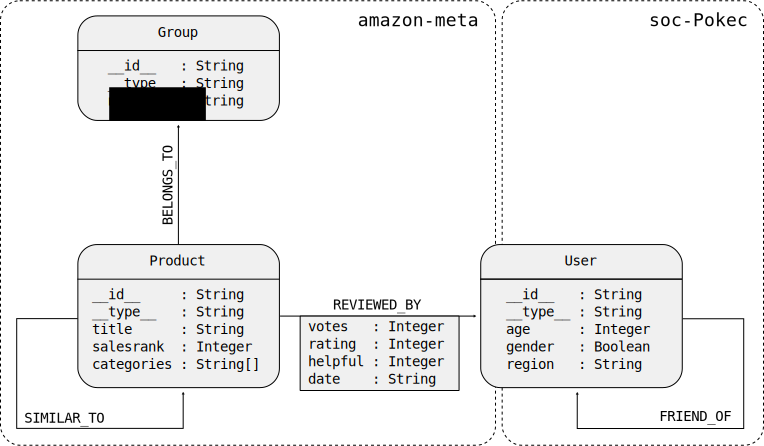
\includegraphics[scale=.75]{schema.pdf}
	\caption[Benchmark: Schema Testdaten]{Schema}
	\label{fig:test}
\end{figure}

\begin{itemize}
	\item Verwendung von ERPNext Schema + Daten (multiplizieren)	
\end{itemize}

\subsection{Testsystem}

\subsection{Methodik}

siehe \cite{Dominguez-Sal2011}

\section{Messungen}

\subsection{Speicherverbrauch}

\subsection{Antwortzeiten}

\begin{itemize}
\item Vergleich Zeichenketten vs. Integer
\end{itemize}

\begin{itemize}
	\item Formulieren verschiedener einfacher und komplexer Anfragen
	\begin{itemize}
		\item Auswahl zuf�lliger Knoten und Abfragen aller Nachbarn bis Tiefe n
		\item Berechnung des Profits in bestimmten Zeitr�umen / Regionen
		\item Auswahl zwei zuf�lliger Knoten vom Typ User, Invoice + Berechnen aller Pfade
		\item ...
	\end{itemize}
\end{itemize}

\section{Ergebnisse}


\chapter{Zusammenfassung, Fazit und Ausblick}

% Blick in Bachelorarbeit

% Zusammenfassung
- Ziel war es ...

% Theoretische Grundlagen
- Nach der Diskussion verwandter Arbeiten in Kapitel x wurden zun�chst die f�r die Arbeit relevanten graphentheoretischen Begriffe definiert.
- graphentheoretische Grundlagen (Definitionen)
- Anwendungszenarien / Arten von Netzwerken -> Schwerpunkt auf Informations- und Wissensnetzwerke
- Die Betrachtung verschiedener Netzwerkarten hat verdeutlicht, dass es graphenbasierte Softwaresysteme mit verschiedenen Schwerpunkten geben muss ...

- Top Down Prinzip!: graphenbasierte Softwaresysteme -> Graphdatenbanksystemen -> Vorauswahl -> funktionaler Vergleich -> Auswahl -> Benchmark

- Kategorisierung: Graphdatenbanksysteme, Graph Processing Systems, Analyse- und Visualisierungssoftware
	- weiter auf GDBMS eingegangen -> Definition und weitere Unterteilung
		- Def: OLTP-artig (Mehrbenutzerf�higkeit, transaktionale Performance, Integrit�t, Verf�gbarkeit)
			- nativ / nicht-nativ
			- zentral / verteilt
			- eingebettet / Client-Server
			- disk- / hauptspeicherzentriert
			
- Datenmodelle (betrachtet: PGM, PHGM, RDF)
	- PGM: gerichteter, kantenbezeichneter, attributierter Multigraph
		- flexibel -> f�r viele Anwendungsf�lle einsetzbar
		- Verantwortung bzgl. Schemaverwaltung an Anwendung �bergeben
		- semistrukturierte Daten (Schemaevolution) -> Integration heterogener Datenquellen
	- PHGM: Erweiterung um n-�re Beziehungen .. seltenes, sehr spezielles Datenmodell
	- RDF in Verbindung mit SPARQL:
		- Schwerpunkte Inferenz und virtuelles Integrieren entsprechen nicht den Schwerpunkten des Forschungsvorhabens
		- fehlende modellinh�rente Differenzierung in eine Beziehung zwischen Ressourcen und einer Beschreibung einzelner Ressourcen zwischen Attribut und Beziehung erschwert das Formulieren analytischer Anfragen
		- keine dynamischen Pfadinstanzen
	-> PGM und (P)HGM f�r das Forschungsvorhaben geeignet
	
- Operationen:
	- grundlegend: 
		- CRUD zur Definition, Manipulation und Auslesen der Datenbasis
		- Traversierung: Beschreiben abstrakter Wege, Grundlage f�r komplexere Operationen
	- komplexe Operationen:
		- Erreichbarkeit: Pfade beliebiger und fester L�nge, k�rzeste Pfade
		- Mustersuche: exakt / inexakt (Unterscheidung in Isomorphismus und Subgraphisomorphismus / Subgraphhomomorphismus)
		- Aggregation als nutzdatenbasiertes Zusammenfassen: insbesondere f�r die analytische Anwendung interessant
		- Summierung als topologisches Zusammenfassen
		- Metriken (zur Analyse des gesamten Graphen) werden in den verglichenen Systmen nicht direkt unterst�tzt und m�ssen bei Bedarf hinzugef�gt werden
		
% Funktionaler Vergleich

- Beschreibung des Forschungsvorhabens:
	- Integration von Unternehmensdaten aus verschiedenen Gesch�ftsinformationssystemen in Graph
	- anschlie�ende Extraktion und Analyse von Teilgraphen
	- Projektziele:
		- (1) Integration
		- (2) Analyse
		- (3) Nutzbarkeit f�r Analysten
		-> (1) und (2) wichtig bei der Betrachtung von GDBMS
		
- Vorauswahl
	- grundlegende Anforderungen nach Kategorien geordnet
	- aus 22 Systemen wurden vier f�r die detaillierte Analyse ausgew�hlt
	- Auff�lligkeiten:
		- wenig hauptspeicher-zentrierte GDBMS
		- Partitionierung des Graphen nur selten unterst�tzt
		- anwendungsseitige Schemaverwaltung

- funktionaler Vergleich
	- Neo4j, HyperGraphDB, OrientDB, Titan
	- der Vergleich hat ergeben, dass ich insbeondere Neo4j und Titan f�r den Einsatz im Forschungsvorhaben eigenen und wurden daher im nachfolgenden Benchmark evaluiert
	
% Benchmark
- hat ergeben, dass
- bei der Verwendung der Datens�tze \texttt{p\_100} und \texttt{p\_1K} konnte kein auff�llig schlechteres Leistungsverhalten des nicht-nativen GBDMS Titan festgestellt werden

% Fazit

Die vier Systemen wurden bereits am Ende von Kapitel \ref{cha:evaluation} verglichen,... Neo4j und Titan wurden auf Grundlage dieses Vergleichs f�r den Benchmark ausgew�hlt und werden im anschlie�enden Fazit bewertet

\paragraph*{Fazit}

- Neo4j
-------
	(1) Integration:
		- PGM, kein Schema, Speicherung semistrukturierter Daten, keine Beeinflussung bestehender Daten
		- Erweiterungen: 
			- Knotenbezeichner -> Schritt in Richtung Entkopplung von der Anwendung + M�glichkeiten zur Anfrageoptimierung

	(2) Analyse:
		- gr��ter Funktionsumfang f�r die Verarbeitung des hinterlegten Graphen
		- Core API, Traversal Framework, Cypher und Gremlin
		- CRUD, Traversierung, Erreichbarkeit, Mustersuche, Aggregation	
		- eigene Algorithmen inkl. Filterkriterien -> z.B. shortestPath sehr gute Performance auch bei steigendem Datenvolumen (verwendbar in Core API und Cypher)
		- Cypher: 
			- steile Lernkurve
			- deutlicher Leistungsunterschied im Vergleich zu Gremlin innerhalb von Neo4j
			- Definition von Graphen innerhalb der Anfrage sehr intuitiv
			- f�r Nicht-Programmierer geeignet
			- Aggregation, Gruppierung, Projektion (+ Funktionen)
			- erm�glicht systemseitige Anfrageoptimierung
			- eventuell Grundlage f�r die Definition einer standardisierten Anfragesprache f�r GDBMS
	
	(3) Speichersystem / Cacheverwaltung
		- einziges natives System (Store-Konzept erm�glicht Trennung von Topologie und Nutzdaten)
		- indexfreie Adjazenz auch physisch umsetzbar
		- im Vergleich erzielte Neo4j in allen Datens�tzen die niedrigsten Antwortzeiten
		- sehr gute Caching- und Persistenzarchitektur
		- skaliert linear bei topologischen Anfragen
		- Probleme beim Pr�fen der Erreichbarkeit, Limitierung durch Hardware

	(4) Erweiterbarkeit:
		- Quelloffenheit erm�glicht generell das Erweitern der GDBMS
		- Implementierung eigener Algorithmen mittels Core API
		- Hinzuf�gen von Indexstrukturen
		
	(5) Verteilung / Skalierbarkeit
		- Replikation erm�glicht Skalierbarkeit von Lesezugriffen (vorteilhaft f�r analytische Anwendung)
		- keine Partitionierung: Datenmenge momentan durch Hardwareressourcen einzelner Rechner limitiert
	
	- objektive Faktoren
		- PGM-Erweiterung um Knotenlabel ist sinnvoll f�r Anfrageoptimierung und Anwendungsmodellierung
		- Cypher leistungsf�hige, deklarative Anfragesprachen f�r die Analyse von Graphen
			- einfaches, intuitives Formulieren graphenbasierter Anfragen
			- Einbettung von Cypher im Quellcode -> hoher Wartungsaufwand (Holzschuher)
			- bei Performance-Problemen (Erreichbarkeit) -> Nutzung der nativen API
		- wenn Gremlin Neo4j 2.0 unterst�tzt, stellt dies ebenfalls eine positive Erweiterung dar (community-driven)
		- eigene Algorithmen / Operationen k�nnen mittels Core API hinzugef�gt werden		-
		- graphenorientiertes Speichersystem und effiziente Caching-Mechanismen
		- bei Bedarf stehen mit Neo4j HA Verteilungsmechanismen zur Verf�gung	
	- subjektive Faktoren
		- umfangreiche, detaillierte, aktuelle Dokumentation
		- gro�e Nutzer- und Entwickler-Community -> viele Projekte, R�ckwirkungen in das Projekt, sehr aktiv
		- offene, erweiterbare Architektur
		- lange Entwicklungsdauer -> fortgeschrittenes Projekt, aktive Community (Unterst�tzung)		
	
- Titan
-------
	(1) Datenmodell:
		- PGM, kein Schema, Speicherung semistrukturierter Daten, keine Beeinflussung bestehender Daten
		- Erweiterungen: 
			- typisierte Attributschl�ssel und Kantenbezeichner (Integrit�tsbedingungen, Festlegung von Datentypen -> effizientere Speicherung + bessere Performance -> konnte im Benchmark nicht festgestellt werden)
			- knoten-zentrierte Indizes (Vorteil in umfangreichen Informationsnetzwerken mit eine Vielzahl von Beziehungsarten und Kantenattributen)
			- mehrfache Verwendung von Attributschl�sseln
	
	(2) Analyse:
		- Blueprints API, Gremlin
		- Gremlin
			- eignet sich sehr gut f�r das Formulieren abstrakter Wege
			- Mustersuche ist m�glich, die Anfrage ist je nach Art des Musters deutlich komplexer als eine �quivalente Cypher-Anfrage
			- (noch) bessere Performance als Cypher
			- Implementierung beliebiger Seiteneffekte durch Java bzw. Groovy
			- imperativ: Performance ist stark von Anfrageformulierung abh�ngig
			
	(3) Speicherung
		- Entkopplung von Datenbankschicht und Speichersystem ist ein innovativer Ansatz und erm�glicht die Implementierung eigener, spezialisierter Speichersysteme bzw. die Bindung an solche
		- keine Trennung von Topologie und Nutzdaten, jedoch direkter Attributzugriff m�glich -> Benchmark hat gezeigt, dass der direkte Zugriff auf Attribute dennoch sehr effizient erfolgt und kurze Antwortzeiten erreicht werden
		- physische indexfreie Adjazenz vom Speichersystem abh�ngig, BerkeleyDB -> logarithmisch
		- Verwendung von BerkeleyDB als Speichersystem f�hrte bei steigender Datenmenge zu teilweise deutlichen Erh�hung der Antwortzeiten
		- skaliert linear bei topologischen Anfragen
		
	(4) Erweiterbarkeit
		- Implementierung eigener Algorithmen mittels Blueprints API
		
	(5) Verteilung / Skalierbarkeit
		- durch Verwendung von entsprechenden Speichersystemen kann sowohl Replikation als auch Partitionierung realsiert werden
		- Partitionierung in Cassandra per Hashfunktion, keine Erhaltung logischer Adjazenz garantiert
		
	- objektiv
		- gut strukturiert, aktuelle Dokumentation, fehlende Dokumentation der internen Abbildung des Graphen
		- R�ckwirkung: die im Zusammenhang mit dem Datenmodell beschrieben Analogie zur Kardinalit�t in Bezug auf UNIQUE-Bedingungen an Kanten wurde in die offizielle Dokumentation �bernommen

- beide
	- Projektziele:
		- (1) Integration -> - Verwaltung semistrukturierter Daten eignet sich im besonderen Ma�e f�r die Integration aus verschiedenen Gesch�ftsinformationssystemen
		- (2) graphenorientierte Analyse -> vielf�ltige Zugriffsmechanismen, Cypher und Gremlin f�r analytische Anfragen geeignet
	- analytische Anfragen m�glich (Cypher, Gremlin)
	- Gremlin
		- h�herer Aufwand bei der Anfrageformulierung
	- standardisierte Anfragesprache fehlt weiterhin
	- Gremlin/Blueprints bildet Quasi-Standard
		- Anpassung der GDBMS-Wrapper ist Community-driven (verz�gert)
	- keine Bestrebungen hinsichtlich Standardisierung erkennbar
	- Cypher ist guter Kandidat f�r Standard
	
	
- R�ckwirkung auf Dokumentationen (OrientDB Transaktionen, Titan Kardinalit�t. Neo4j Anfragebeispiele)

% Ausblick
\paragraph*{Ausblick}

- Neo4j:
	- In-Memory-Erweiterungen f�r Analyse
	- Query-Optimierung
	- formale Untersuchung und Standardisierung von Cypher im GDBMS-Sektor
	- ausf�hrlicher Benchmark (parallele Queries, reale Unternehmensdaten)
	- Partitionierung
	- Ergebnis der Cypher-Anfragen ist Tabelle und kein Graph bzw. Graphmenge -> �nderungen?
	- Clustering im Speichersystem -> Abbildung einer logischen auf eine physische Adjazenz
	
- OrientDB
	- neues Speichersystem evaluieren
- HyperGraphDB
	- Implementierung Blueprints API
	
- quelloffene hauptspeicher-zentrierte Implementierung
- Eignung Graph Processing f�r Forschungsvorhaben
- Visualisierung f�r Analyseplattform

- Benchmark
	- Import: lesen und Schreiben von einer Platte (unrealistisch)
	- parallele Lesezugriffe
	- warmup-Prozedur verhindert Feststellen der Leistungsf�higkeit des Speichersystems
	-> weiterf�hrende Benchmarks
	- Betrachtung ohne Caches sinnvoll?

\chapter{Zusammenfassung und weitere Entwicklung}
\label{cha:Fazit}

- OrientDB neues Speichersystem effizienter?
- HyperGraphDB -> Implementierung Blueprints API
- hauptspeicher-zentrierte Implementierung

- analytische Anfragen m�glich (Cypher, Gremlin)

- R�ckwirkung auf Dokumentationen (OrientDB Transaktionen, Titan Kardinalit�t)

% Literaturverzeichnis -----------------------------------------------------
%		Das Literaturverzeichnis wird aus der Datenbank Bibliographie.bib 
% 		erstellt. Die genaue Verwendung von bibtex wird hier jedoch nicht erkl�rt.
%		Link: http://de.wikipedia.org/wiki/BibTeX
% --------------------------------------------------------------------------
\bibliography{quellen}
\bibliographystyle{plain}
% \bibliographystyle{natdin}		% DIN-Stil des Literaturverzeichnisses
% \bibliographystyle{geralpha}


%\pagenumbering{gobble}
\addchap{Erkl�rung}
Ich versichere, dass ich die vorliegende Arbeit mit dem Thema:

\begin{center}
\textit{\glqq\titel\grqq}\\[1em]
\end{center}
			
selbst�ndig und nur unter Verwendung der angegebenen Quellen und Hilfsmittel angefertigt habe, insbesondere sind w�rtliche oder sinngem��e Zitate als solche gekennzeichnet. Mir ist bekannt, dass Zuwiderhandlung auch nachtr�glich zur Aberkennung des Abschlusses f�hren kann.
\par
\ort, den \eingereicht


\rule[-0.2cm]{5cm}{0.5pt}

\textsc{\autor} 
	% Selbst�ndigkeitserkl�rung 

% Anhang -------------------------------------------------------------------
%		Die Inhalte des Anhangs werden analog zu den Kapiteln inkludiert.
%		Dies geschieht in der Datei Anhang.tex
% --------------------------------------------------------------------------
\begin{appendix}
	\clearpage
	\pagenumbering{roman}
	\chapter{Anhang }
\label{cha:Anhang}

\section{GDBMS-Implementierungen}
\label{anh:vendor_list}

blbla
\end{appendix}


% Index --------------------------------------------------------------------
%		Zum Erstellen eines Index, die folgende Zeile auskommentieren.
% --------------------------------------------------------------------------
%\printindex		% Index hier einf�gen
%\ofoot{}
%\include{Inhalt/Thesen}	% Thesen 

\end{document}
